% Generated from MANUSCRIPT.md and SUPPLEMENTARY.md; saved numerical outputs unchanged.
% Compile twice with pdfLaTeX, or use latexmk -pdf manuscript.tex.
% Bibliography is embedded: no BibTeX/Biber step is required.
\documentclass[11pt,a4paper]{article}
\usepackage[margin=25mm]{geometry}
\usepackage[T1]{fontenc}
\usepackage[utf8]{inputenc}
\usepackage{lmodern,microtype}
\usepackage{amsmath,amssymb}
\usepackage{graphicx}
\usepackage{booktabs,tabularx,array,longtable,pdflscape}
\usepackage{caption}
\usepackage[super,numbers,sort&compress]{natbib}
\usepackage[hyphens]{url}
\usepackage[hidelinks]{hyperref}
\hypersetup{pdftitle={Contact-network remodeling during bacterial sheath contraction},pdfauthor={Anthony Yua Ior}}
\captionsetup{font=small,labelfont=bf}
\setlength{\parindent}{1.2em}
\setlength{\parskip}{0.35em}
\setlength{\emergencystretch}{2em}
\renewcommand{\bibsection}{\section*{References}}
\setlength{\bibsep}{0.5em}


\title{Contact-Network Remodeling During Bacterial Sheath Contraction Is Associated with Site-Specific Evolutionary Rates in an AFP System}

\author{Anthony Yua Ior\thanks{Correspondence: \href{mailto:ior23@itu.edu.tr}{ior23@itu.edu.tr}.}\\[0.5em]
\small Istanbul Technical University\\
\small Maslak 34867, Istanbul, Turkiye}
\date{}
\begin{document}
\maketitle
\begin{abstract}

\textbf{Background:} Bacterial contractile injection systems undergo substantial conformational rearrangements, but the evolutionary relevance of residue-level contact-network remodeling remains unclear.

\textbf{Objectives:} To test whether remodeling is associated with site-specific evolutionary rates after adjustment for monomer solvent accessibility, packing and flexibility averaged across extended and contracted states.

\textbf{Methods:} We quantified remodeling in five sheath proteins from four systems, constructed positional-orthology datasets for three proteins from two systems, estimated relative rates with Rate4Site, and fitted protein-specific multiple linear regressions using the archived state-averaged monomer descriptors. Sequence-block bootstrap intervals used contiguous ten-residue reference windows.

\textbf{Results:} Positive adjusted associations were detected in AFP Afp2 (standardized \(\beta_R\) = +0.435; sequence-block bootstrap 95\% confidence interval [CI], +0.229 to +0.636) and Afp3 (+0.425; +0.281 to +0.544). On variable sites, the Afp3 association remained positive (+0.355; +0.189 to +0.490), whereas the Afp2 interval included zero (+0.275; \ensuremath{-}0.023 to +0.545). No association was detected in diffocin (+0.035; \ensuremath{-}0.173 to +0.244).

\textbf{Conclusion:} Evidence that remodeling contains additional evolutionary-rate information is strongest in Afp3 and less robust in Afp2. Diffocin's narrower remodeling range and greater relative rate uncertainty prevent confident biological attribution of the between-system contrast. The evidence concerns two systems, with two non-independent AFP proteins. Sequence-block intervals do not explicitly account for three-dimensional structural dependence.

\end{abstract}

\noindent\textbf{Keywords:} contractile injection system; sheath contraction; protein evolution; site-specific evolutionary rate; intermolecular contacts; structural remodeling.

\section{Introduction}

Bacterial contractile injection systems convert the energy stored in an extended protein sheath into mechanical work. A helical sheath surrounds an inner tube and connects to a baseplate; contraction shortens and widens the sheath, driving the tube and its distal tip toward a target cell. In bactericidal systems such as R2 pyocin, membrane penetration can kill the target, whereas the \emph{Serratia entomophila} antifeeding prophage (AFP) uses a related apparatus for toxin delivery to an insect host.\cite{ref1,ref2} The sheath is therefore both a structural assembly and the force-generating component of the machine, making the interactions that maintain its two conformations relevant to its function. For a sheath residue, functional constraint may arise from compatibility with the extended assembly, the contracted assembly, or the transition between them. This distinction motivates an evolutionary description that considers the identities of contacts across states, rather than describing the local environment in only one structure.

Cryo-electron microscopy has established how these assemblies change during contraction. Atomic models of extended and contracted R2 pyocin reveal subunit reorientation within an interwoven sheath whose connecting arms maintain the overall mesh.\cite{ref1} AFP structures resolve the distinct Afp2 and Afp3 sheath proteins and the intersubunit interaction networks accompanying contraction.\cite{ref2} Structures of the \emph{Clostridioides difficile} bacteriocin diffocin and the \emph{Salmonella enterica} subsp. \emph{salamae} contractile injection system (SalCIS) extend this structural comparison to different sheath architectures and contraction geometries.\cite{ref3,ref4} These paired conformations allow the contacts retained, lost or gained by an individual residue to be identified directly. Retention of an overall sheath mesh does not imply that every atomic contact is retained. Assembly connectivity and residue-level contact identity describe different levels of organization: a connected interface can remain intact while its constituent contacts change as subunits reorient.

Protein structure already provides a strong basis for understanding why amino-acid substitution rates vary among sites. Solvent-exposed residues generally evolve faster than buried residues, while densely packed positions tend to be more constrained. Analyses of residue microenvironments identify solvent accessibility and packing as rate predictors, although their relative contributions depend on the dataset and descriptor.\cite{ref5,ref6} Structural flexibility also correlates with site-specific evolutionary variation, but its relationship with packing means that these descriptors need not represent independent constraints. Elastic-network analyses connect both properties to the perturbation of an active conformation by mutation, and show that the rate--flexibility relationship need not be linear.\cite{ref7} Accessibility, packing and flexibility thus provide appropriate baseline descriptors against which to assess an additional structural property.

These descriptors do not, however, directly encode the identity of intermolecular contacts exchanged between functional states. Even when monomer descriptors are averaged across conformations, they summarize local exposure, packing or fluctuation rather than contact partner identity. A residue can retain similar burial or packing while changing its interaction partners, and small fluctuations around one conformation differ from the collective rearrangement of an assembled sheath. Interface involvement itself is associated with evolutionary constraint,\cite{ref5} but describing an interface in one state does not establish whether its remodeling during contraction carries additional rate information. We hypothesize that contact exchange captures constraints associated with maintaining the sheath's conformational transition that are incompletely represented by conventional monomer descriptors. This hypothesis does not prescribe the direction of the association: persistent and remodeled contacts could each impose functional constraints.

We investigated whether residue-level remodeling of intermolecular contact networks during sheath contraction is associated with site-specific evolutionary rates beyond variation explained by solvent accessibility, intramolecular packing and intrinsic flexibility. We quantified remodeling across four bacterial systems and estimated rates with Rate4Site for AFP Afp2, AFP Afp3 and diffocin, where positional evidence supported interpretable sequence correspondence.\cite{ref8,ref9} We tested a non-directional adjusted linear relationship using protein-specific multiple linear regression models, while allowing local sequence dependence in uncertainty estimation. The study asks whether remodeling contributes information conditional on the conventional monomer descriptors averaged across states; it does not establish causality or treat the two AFP proteins as independent system-level replicates.

\section{Materials and Methods}

\subsection{Structural systems and residue mapping}

The five sheath references comprise R2 pyocin of \emph{Pseudomonas aeruginosa},\cite{ref1} AFP Afp2 and Afp3 of \emph{Serratia entomophila},\cite{ref2} the \emph{Clostridioides difficile} diffocin sheath CD1363,\cite{ref3} and the \emph{Salmonella enterica} subsp. \emph{salamae} SalCIS sheath.\cite{ref4} Experimentally determined extended and contracted states, adequate surrounding sheath neighbours and interpretable cross-state residue correspondence defined the retained structural set (Table~\ref{tab:structures}). AFP contributes two proteins within one system.

\begin{table}[htbp]
\centering
\caption{Structural datasets. Extended (E) and contracted (C) PDB entities identify the five sheath references. Example author chain identifiers are case-sensitive deposited family members; selected contact-reference subunit keys were not archived.}
\label{tab:structures}
\footnotesize
\setlength{\tabcolsep}{3pt}
\renewcommand{\arraystretch}{1.25}
\begin{tabularx}{\textwidth}{@{}>{\raggedright\arraybackslash}X>{\raggedright\arraybackslash}p{0.10\textwidth}>{\raggedright\arraybackslash}p{0.15\textwidth}>{\raggedright\arraybackslash}p{0.15\textwidth}>{\raggedright\arraybackslash}p{0.16\textwidth}r@{}}
\toprule
\textbf{System} & \textbf{Protein} & \textbf{Extended PDB/entity} & \textbf{Contracted PDB/entity} & \textbf{Example author chains, E/C} & \textbf{Eligible sites} \\
\midrule
R2 pyocin & Sheath & 3J9Q/1 & 3J9R/1 & A/A & 143 \\
AFP & Afp2 & 6RBN/2 & 6RC8/1 & C/A & 84 \\
AFP & Afp3 & 6RBN/3 & 6RC8/2 & D/B & 82 \\
SalCIS & Sheath & 9R9H/1 & 9R9I/1 & T/O & 68 \\
Diffocin & CD1363 & 8V3X/1 & 8V3Y/1 & g/B & 58 \\
Total &  &  &  &  & 435 \\
\bottomrule
\end{tabularx}
\end{table}

Chain identifiers in Table~\ref{tab:structures} identify deposited family members and are case-sensitive; they do not substitute for the selected interior contact-reference subunit. The reference selection algorithm and all deposited chain sets are documented in Table~\ref{tab:supp1}. The selector first prefers interior-ring subunits, then maximizes the number of assembly centroids within 90 \AA{}; ties retain the first candidate in input order. Original mmCIF files, selected keys and tie-candidate scores are absent from the retained archive. Therefore, the algorithm is specified but the exact previously used subunits cannot be verified from the archived outputs alone. A procedure and input audit accompany the supplement; no unsupported reference-chain identifier is assigned.

Modeled standard amino acids carrying C\ensuremath{\alpha} atoms were aligned between states using global BLOSUM62 alignment (gap opening \ensuremath{-}11; extension \ensuremath{-}1). Families required at least 90\% identity among modeled sequences. Aligned positions were assigned a shared canonical index; the extended modeled sequence was separately aligned to the deposited entity SEQRES to obtain one-based reference positions. Unresolved positions were not reconstructed, and contacts to partner positions without cross-state correspondence were excluded symmetrically. The retained continuous-metric producer does not implement the earlier categorical pilot's 8 \AA{} engineering shell. No such exclusion is claimed for the continuous analysis. Cross-state sequence identity and modeled coverage are reported in Table~\ref{tab:supp1}.

\subsection{Contact-network remodeling}

A contact joins a focal residue to a residue in a different protein subunit when their minimum heavy-atom distance is strictly less than 5.0 \AA{}. Its identity is the tuple (partner family, relative ring, relative azimuth, canonical partner residue). Ring and azimuth labels come from the coordinate-derived sheath lattice, with relative azimuth calculated modulo the inferred subunits-per-ring value. Contacts with the same tuple in both states are shared even if their distances differ below the cutoff.

\begin{equation}
R_i=1-\frac{\lvert C_i^E\cap C_i^C\rvert}{\lvert C_i^E\cup C_i^C\rvert}.
\label{eq:remodeling}
\end{equation}

where \(C_E\) and \(C_C\) are the residue's extended and contracted contact sets. A union of at least three distinct contact identities defines eligibility. \(R_i\) = 0 denotes no detected contact-set remodeling and \(R_i\) = 1 denotes no shared contacts. A three-contact set in each state with two shared identities has four contacts in the union and \(R_i\) = 0.5. The domain rule limits unstable comparisons of very sparse contact sets; it does not make the metric a measure of force, energy or functional importance.

R2 pyocin, SalCIS and diffocin use deposited coordinate copies. AFP requires the deposited biological-assembly operators to expand its asymmetric-unit chains in both states; these operator-derived copies are distinguished from guessed ring-completion subunits. None of the five retained protein references required ring completion. The recorded zero ring-completion dependence should therefore not be described as absence of all generated coordinates in AFP. Contact-definition QC and the explanatory metric schematic are provided in Figure~\ref{fig:supp1}. The manuscript uses the retained structural measurements.

\subsection{Evolutionary sequence retrieval and orthology}

Bacterial UniProtKB sequences from release 2026\_03 (2 September 2026) were retrieved using Pfam signatures attached to the reference entries.\cite{ref10,ref11} The deposited reference sequence anchored the structural-to-evolutionary comparison. Local BLAST+ blastp 2.17.0+ supplied candidate similarity evidence.\cite{ref12} The recorded single-query filters were E \ensuremath{\leq} \(10^{-5}\), 30--90\% identity, at least 80\% reference coverage and a 0.75--1.30 length ratio, followed by highest-bitscore species dereplication. AFP additionally used a joint family prescreen and subfamily-specific positional analysis; its archived funnel is reported separately rather than assigning unrecorded per-query counts.

Sequence similarity could not distinguish AFP's tandem sheath genes. Positional assignment used non-sheath flanking-gene homology, conserved orientation and collinear gene order in \ensuremath{\pm}25 kb neighbourhoods. At least three non-sheath anchors, a modal-offset share of at least 60\%, and Spearman collinearity \ensuremath{\rho} \ensuremath{\geq} 0.8 when defined determined anchoring. Unanchored loci remained unassigned. A joint orthology-assessment phylogeny provided an independent diagnostic of positional labels; it did not replace locus assignment. The detailed procedure, AFP subfamily restriction and exclusion evidence for R2 pyocin and SalCIS are provided in Supplementary Methods and Figures S2--S4.

Both ambiguous \emph{Peptacetobacter hiranonis} diffocin copies were excluded from the primary 33-sequence dataset before rate estimation. The screened 35-sequence and collinear-frame 66-sequence datasets were retained as sensitivity sets. R2 pyocin was excluded because coexisting divergent copies could not be assigned reliably to one reference lineage; SalCIS was excluded because reference-locus recovery was inadequate. Neither exclusion was based on fitted rate associations.

\subsection{Multiple sequence alignments and phylogenetic inference}

Datasets were aligned with FAMSA through pyfamsa 0.7.0.\cite{ref13} Each alignment included its structural reference as \path{REF}; the ungapped row matched the deposited SEQRES exactly. No additional alignment-column trimming is documented for these final inputs. Reference positions were mapped to non-gap \path{REF} columns, and structural sites with less than 80\% non-gap occupancy were omitted from regression. This removed one Afp3 site, yielding the fitted counts in Table~\ref{tab:datasets}.

Final phylogenies used IQ-TREE 3.1.4,\cite{ref14} ModelFinder with BIC selection,\cite{ref15} maximum-likelihood branch-length optimization, 1,000 ultrafast bootstrap replicates\cite{ref16} and 1,000 SH-aLRT replicates.\cite{ref17} Selected primary models were WAG+I+G4 for both AFP proteins and LG+F+I+G4 for diffocin. The final topologies, with support labels removed for input compatibility, were supplied to Rate4Site. The FastTree LG+\ensuremath{\Gamma} trees used for orthology assessment were not used for primary rate estimation. Alignment and phylogenetic summaries appear in Table~\ref{tab:supp3}; exact commands are retained in the supplementary evidence archive.

\subsection{Evolutionary-rate estimation}

Rate4Site self-reported version 2.01 and used empirical Bayes estimation with WAG+\ensuremath{\Gamma} and 16 discrete rate categories.\cite{ref8,ref9,ref18} WAG was the best available implemented matrix in the primary datasets; LG was unavailable. Rate4Site reoptimized branch lengths under its own model on the fixed IQ-TREE topology. The source-build provenance and model mismatches for the alternative diffocin datasets are documented in Supplementary Methods.

Larger normalized output scores indicate faster relative evolution. The increasing relationship to unnormalized posterior rates was checked in every dataset (Spearman \ensuremath{\rho} \ensuremath{\geq} 0.999). Invariant sites were retained in the primary models and received empirical Bayes estimates; they were not assigned one common fixed rate floor. Rates are relative amino-acid substitution rates, not absolute rates or dN/dS estimates. Site-specific posterior uncertainty was retained for descriptive reporting but was not propagated into regression uncertainty.

\subsection{Structural covariates}

RSA was computed for the monomer with the Shrake--Rupley algorithm\cite{ref19} and normalized by the theoretical maximum solvent-accessible areas of Tien et al.\cite{ref20} WCN summed inverse squared C\ensuremath{\alpha} distances to all other modeled residues of the same chain; self-pairs were excluded, and adjacent sequence neighbours were included without a sequence-separation exclusion.\cite{ref6} GNM used a 7.3 \AA{} C\ensuremath{\alpha} cutoff, a Kirchhoff matrix of monomer contacts, and the diagonal of its pseudoinverse as the fluctuation statistic.\cite{ref21}

The fitted predictors are the saved \path{rsa}, \path{wcn} and \path{gnm} columns. For each matched position, the retained producer computes each descriptor on representative isolated monomer chains in the extended and contracted structures, then writes the arithmetic mean of available state values. This is an average of descriptor values, not a calculation on averaged atomic coordinates. The representative monomer chains used for these calculations are distinct from the interior subunit selection used to measure assembly contacts. RSA, WCN and GNM in the regression refer throughout to these state-averaged inputs.

Averaging describes the residue's monomer environment across the two observed states, while remodeling describes exchange of intermolecular contact identities. These remain different measurements, but the averaging determines the conditional comparison: \(\beta_R\) is adjusted for state-averaged monomer properties. The written specification instead called for extended-state-only covariates. We retain that record and disclose the mismatch as an implementation departure, not a correction of the planned estimand. State-specific intermediate values were not preserved. No state was chosen after inspecting associations, and no model was refitted; an extended-state-only adjusted association has not been tested.

\subsection{Primary linear regression}

The primary dataset definitions, model form and uncertainty procedure were specified in writing before rate estimation. The analysis tested a non-directional association and retained separate models for the three proteins. For each protein,

\begin{equation}
\boxed{\begin{aligned}
z(r_i)=\beta_0 &+\beta_R z(R_i)+\beta_A z(\mathrm{RSA}_i)\\
&+\beta_P z(\mathrm{WCN}_i)+\beta_F z(\mathrm{GNM}_i)+\varepsilon_i .
\end{aligned}}
\label{eq:regression}
\end{equation}

where \(r_i\) is the estimated site rate, \(R_i\) is contact remodeling, and RSA, WCN and GNM are the three monomer descriptors averaged across the available states. The outcome and each predictor were standardized within the protein using the sample SD. The primary estimand, \(\beta_R\), is the adjusted change in standardized rate associated with a one-SD increase in remodeling, holding the three covariates constant. Ordinary least squares estimates this conditional linear association; it does not specify the complete biological functional form. No interactions, nonlinear terms, variable selection or pooled primary model were fitted.

The reduced model contains RSA, WCN and GNM but excludes remodeling. Incremental explanatory value is quantified by

\begin{equation}
R^2_{\mathrm{partial},R}=\frac{R^2_{\mathrm{full}}-R^2_{\mathrm{reduced}}}{1-R^2_{\mathrm{reduced}}}.
\label{eq:partialr2}
\end{equation}

This is the fraction of variation unexplained by the reduced model that is additionally accounted for by remodeling; it is not the proportion of total rate variance explained. Variance inflation factors describe linear redundancy among predictors. Full coefficients, standard errors, independent-site OLS intervals and VIFs appear in Table~\ref{tab:supp4}.

\subsection{Uncertainty estimation}

We report independent-site OLS intervals separately from percentile sequence-block bootstrap intervals. The latter are the interval estimates emphasized in the interpretation. Bootstrap resampling\cite{ref22} was applied to sequence blocks to retain some local dependence, consistent with the motivation for block resampling of dependent observations.\cite{ref23} The implementation is a fixed-window site bootstrap, rather than a claim to reproduce all assumptions of a stationary time-series bootstrap.

Windows comprise reference positions 1--10, 11--20 and so forth. Only windows containing fitted sites form the sampling pool, with 1--10 eligible sites per window. There are 26 blocks for Afp2, 23 for Afp3 and 17 for diffocin. Blocks were sampled with replacement until at least the original site count was reached, with excess rows from the final sampled block truncated. Predictors and outcome were re-standardized in each of 10,000 replicates; the 2.5th and 97.5th slope percentiles form the 95\% interval. This allows local sequence dependence within windows but does not necessarily account for residues that are distant in sequence and adjacent in three-dimensional structure. Interval coverage under that remaining dependence was not assessed, so these intervals are not spatially corrected or a complete adjustment for residue dependence. They are conditional on the retained structures, orthology assignments, rate point estimates and fitted sites; sequences, phylogenies, structural choices and rate posterior uncertainty were not resampled.

\subsection{Sensitivity analyses and prior exposure}

The written sensitivity plan explicitly names the alternative diffocin sequence sets, Afp2's variable-site restriction and occupancy relaxation to 50\%. The saved results also contain analogous variable-site checks for Afp3 and diffocin, extending the literal scope of that clause; these are reported transparently as archived checks rather than claiming that all three restrictions are expressly documented in the written plan. Variable sites contain at least two distinct non-gap amino acids. All saved specifications are listed in Table~\ref{tab:supp5}. No additional fits were introduced for this manuscript revision.

Before the specification, an exploratory R2 pyocin alignment entropy--remodeling correlation was examined (\ensuremath{\rho} = 0.32 and 0.33 in two candidate sets). It was neither adjusted for covariates nor a rate estimate, and R2 pyocin is excluded from the rate analysis. The primary analysis is therefore prespecified from that documented point forward, rather than wholly independent of prior sequence-variability inspection.

\section{Results}

\subsection{Residue-level contact remodeling varies across contractile sheaths}

Across 435 eligible sites, remodeling spans the full range in each of the five protein references (Figure~\ref{fig:remodeling}). Median \(R_i\) is 0.80 in R2 pyocin, 0.58 in SalCIS, 0.50 in Afp2 and Afp3, and 0.236 in diffocin. The fraction with no detected contact-set remodeling ranges from 5\% in R2 pyocin to 33\% in diffocin. Diffocin therefore has comparatively limited remodeling, while contact exchange is heterogeneous within every sheath. Afp2 and Afp3 are separate proteins of one particle, rather than separate system observations.

These distributions describe exchange of interaction partners within the assembled sheath. Subunit reorientation can change residue-level contacts while the interwoven assembly remains connected. The metric therefore concerns the identities of interactions supporting the two observed conformations, without assigning a residue a mechanical or energetic role. The distributions do not localize remodeling on the sheath or describe the transition path.

A zero index does not establish that a residue remains stationary, and a unit index does not measure displacement, force or functional importance. These distributions establish variation in contact-set identity across states; by themselves they are not evidence of evolutionary constraint. The structural sites and state identifiers are listed in Table~\ref{tab:structures}, and detailed mapping and eligibility are provided in Table~\ref{tab:supp1}.

\subsection{Positional orthology determines evolutionary dataset feasibility}

Four systems were assessed, and AFP and diffocin supplied three protein-specific datasets (Figure~\ref{fig:datasets}, Table~\ref{tab:datasets}). R2 pyocin and SalCIS were excluded before rate estimation. The fitted counts sum to 223 sites, representing three protein datasets from two systems.

\begin{table}[htbp]
\centering
\caption{Primary evolutionary datasets. Variable sites contain at least two distinct non-gap amino acids. The 223 fitted sites sum protein-specific samples from two systems, with two AFP proteins in one system.}
\label{tab:datasets}
\footnotesize
\setlength{\tabcolsep}{3pt}
\renewcommand{\arraystretch}{1.25}
\begin{tabularx}{\textwidth}{@{}>{\raggedright\arraybackslash}Xrrr@{}}
\toprule
\textbf{Dataset} & \textbf{Sequences} & \textbf{Sites fitted} & \textbf{Variable sites} \\
\midrule
Diffocin & 33 & 58 & 50 \\
AFP Afp2 & 27 & 84 & 51 \\
AFP Afp3 & 31 & 81 & 64 \\
Total fitted sites &  & 223 &  \\
\bottomrule
\end{tabularx}
\end{table}

Diffocin's 142 sampled loci each contained one detected sheath gene, but seven of 137 replicons carried a second candidate locus. Locus-level copy number consequently did not guarantee genome-level orthology. Both mutually exclusive \emph{P. hiranonis} assignments were removed from the primary set. AFP's two reference proteins are only 38.1\% identical; sequence best-hit labels disagreed with the Afp2 position for 15 of 22 assigned genes in the family-wide locus assessment. Positional correspondence was interpretable within the reference subfamily, where 35 of 42 loci carried a three-gene sheath run and 55 of 58 assigned genes agreed with the sequence comparison. The two AFP datasets were kept separate.

For R2 pyocin, 221 of 967 screened species carried multiple gated candidates, and 39 of 57 discarded paralogs lay within the candidate clade. In 11 of 35 testable pairs the discarded copy recovered reference gene order better than the retained copy. For SalCIS, only the reference among 4,490 BLAST hits was \emph{Salmonella}, and the reference locus could not be anchored in 84\% of sampled loci. These distinct barriers prevented reliable reference-lineage assignment. Detailed locus, copy-number and phylogenetic evidence is confined to Supplementary Figures S2--S4 and Tables S2--S3.

\subsection{Protein-specific adjusted linear associations with evolutionary rate}

Contact remodeling showed a positive adjusted linear association with evolutionary rate in both AFP sheath proteins (Figure~\ref{fig:association}, Table~\ref{tab:primary}). A one-SD increase in remodeling was associated with approximately 0.43 SD faster evolution after adjustment for the three monomer descriptors averaged across states. Remodeling accounted for about 15\% of the variance left unexplained by the covariate-only model, while full-model \(R^2\) was 0.226 for Afp2 and 0.209 for Afp3. Much of the total rate variation remains unexplained.

\begin{table}[htbp]
\centering
\caption{Adjusted remodeling associations and variable-site restrictions. Standardized coefficients describe rate SD per remodeling SD conditional on monomer RSA, WCN and GNM averaged across states. Intervals use ten-reference-position sequence windows; all intervals are sequence-block bootstrap estimates and variable-site documentation scope is explained in the Methods and Table S5.}
\label{tab:primary}
\footnotesize
\setlength{\tabcolsep}{3pt}
\renewcommand{\arraystretch}{1.25}
\begin{tabularx}{\textwidth}{@{}>{\raggedright\arraybackslash}X*{3}{>{\centering\arraybackslash}p{0.205\textwidth}}@{}}
\toprule
\textbf{Quantity} & \textbf{AFP Afp2} & \textbf{AFP Afp3} & \textbf{Diffocin} \\
\midrule
Adjusted \(\beta_R\) & +0.435 & +0.425 & +0.035 \\
Sequence-block-bootstrap 95\% CI & [+0.229, +0.636] & [+0.281, +0.544] & [\ensuremath{-}0.173, +0.244] \\
Partial \(R^2\) & 0.148 & 0.155 & 0.001 \\
Full-model \(R^2\) & 0.226 & 0.209 & 0.121 \\
Variable-site \(\beta_R\) & +0.275 & +0.355 & \ensuremath{-}0.059 \\
Variable-site sequence-block 95\% CI & [\ensuremath{-}0.023, +0.545] & [+0.189, +0.490] & [\ensuremath{-}0.339, +0.234] \\
\bottomrule
\end{tabularx}
\end{table}

Under the same sequence-block resampling scheme, the association remained evident after restricting Afp3 to its 64 variable sites (+0.355; +0.189 to +0.490). For Afp2, the estimate decreased to +0.275 on 51 variable sites and the interval included zero. Its 33 invariant sites are legitimate primary observations, but the restriction weakens evidence among sites displaying observed amino-acid variation. Omitting invariant sites changes the represented site population; it does not establish that the primary result is artifactual.

No comparable association was detected in diffocin (+0.035; \ensuremath{-}0.173 to +0.244). The screened and collinear-frame sets returned +0.071 and +0.121, respectively, with intervals spanning zero. Occupancy relaxation left Afp2 and diffocin unchanged and added one Afp3 site (+0.419; +0.277 to +0.541). Complete saved sensitivity results appear in Table~\ref{tab:supp5}; the documentation distinction for the parallel Afp3 and diffocin variable-site checks is retained there.

Remodeling VIFs ranged from 1.11 to 1.41, indicating limited linear redundancy with the included descriptors, although the conventional descriptors were mutually collinear. This supports interpretation as incremental conditional information, not mechanistic independence. Afp2 and Afp3 are non-independent system-level observations. The results therefore provide a bounded AFP association, strongest in Afp3, rather than three independent confirmations of a general hypothesis.

\section{Discussion}

\subsection{Evolutionary information supplied by contact remodeling}

The principal result is that contraction-associated contact remodeling carries additional site-specific evolutionary-rate information in AFP after adjustment for the included monomer descriptors averaged across states. Structural studies establish that the sheath functions through a collective rearrangement of an interconnected assembly,\cite{ref1,ref2} whereas conventional rate predictors characterize the residue's environment within a conformation.\cite{ref5,ref6} The present comparison brings these descriptions together by asking whether the contacts exchanged between experimentally observed states retain an association with rate after those baseline properties are considered. The answer is positive within the AFP datasets, with the most consistent evidence in Afp3.

Both AFP proteins show positive primary coefficients of approximately 0.43, and remodeling accounts for about 15\% of the variance remaining after the covariate-only adjustment. The full-model \(R^2\) values of 0.21--0.23 make clear that considerable site-level variation remains unexplained. These are in-sample associations. The study neither evaluates prediction on new proteins nor establishes a general quantitative law relating contact exchange to evolutionary rate.

The variable-site restriction distinguishes the contributions of Afp2 and Afp3. Afp3 retains a positive association when invariant columns are omitted, so its result is supported among sites displaying observed amino-acid variation. Afp2's estimate remains positive but decreases, and its interval includes zero. Invariant sites contribute legitimate information about conservation to the primary analysis; omitting them is not intrinsically a superior rate model. Nevertheless, the weaker variable-site result limits the evidence that the Afp2 association extends across the variation among substitution-bearing positions. It also cautions against presenting the similar primary coefficients as equally robust results.

Afp2 and Afp3 belong to the same particle and were sampled within the same enterobacterial radiation. Their agreement is therefore informative within AFP but supplies limited independent replication across biological contexts. The supported conclusion is that contact remodeling is associated with rate in this system, most consistently in Afp3. It is not that two independently sampled contractile systems have demonstrated the same relationship. This distinction is retained in the abstract and Conclusion.

\subsection{Possible constraints across functional states}

The positive sign means that more remodeled AFP residues tend to evolve faster relative to other analyzed residues in the same protein. One possible interpretation is that contacts retained across conformations impose more persistent restrictions on allowable amino acids than contacts present in only one state. An alternative is that remodeled sites tolerate different local interaction solutions while preserving the collective behavior of the sheath. These are hypotheses about how the observed association might arise, not mechanisms demonstrated by the regressions. Contact energies, mutational fitness effects and contraction efficiency were not measured. A rapidly evolving remodeled site can remain functionally important, and a positive rate association does not establish adaptive evolution.

The metric also separates partner identity from contact abundance. A residue may exchange partners without changing its number of contacts, as illustrated in Figure~\ref{fig:supp1}. This provides a specific reason why a state-comparison descriptor can carry information beyond monomer packing or exposure. However, the fitted coefficient establishes incremental information conditional on the chosen descriptors, rather than mechanistic independence. Remodeling could covary with an unmeasured feature of the assembled interface, and the present models do not identify which physical property mediates the relationship.

\subsection{Interpreting non-detection in diffocin}

No adjusted association was detected in diffocin under the primary analysis or any reported sensitivity specification. Repeating the analysis on the screened dataset and the larger collinear-frame set shows that the conclusion is not determined by the single primary dataset definition. The intervals nevertheless include effects of potentially meaningful magnitude. These estimates delimit what the available data can resolve; they do not establish an absence of evolutionary constraint associated with remodeling.

Two properties of the existing data complicate the AFP--diffocin comparison. First, diffocin has a narrower remodeling distribution, with 19 of 58 fitted sites at zero and an SD of 0.305, compared with 0.383 and 0.393 in AFP. For a common slope in original units and comparable residual variation, a narrower predictor range can reduce both the standardized association and the ability to detect it. Second, the median Rate4Site posterior SD is 42\% of the between-site rate SD in diffocin, compared with 31\% in Afp2 and 27\% in Afp3. These relative uncertainties and remodeling distributions are displayed in Figure~\ref{fig:supp5}. They are descriptive features of the saved estimates, not a formal power analysis or a measurement-error correction.

Diffocin has greater effective genus breadth and a higher proportion of variable structural sites than AFP. Those summaries do not suggest a simple shortage of sequence diversity, but diversity alone does not determine the precision of a conditional site-level association. In particular, adding sequence diversity cannot guarantee a wider structural predictor range or eliminate uncertainty in estimated rates. It would therefore be too strong to attribute the contrast to biology after excluding sampling or estimation limitations on the basis of these summaries.

Biological differences remain plausible. AFP and diffocin differ in sheath architecture, biological targets and the organization of their sheath genes.\cite{ref2,ref3} Such differences may change which interactions constrain assembly or function. However, no formal between-system effect comparison was prespecified, and a detected association in AFP combined with non-detection in diffocin is not itself evidence that their underlying effects differ. The present analysis cannot separate contextual biology from differences in predictor variation and relative rate uncertainty.

\subsection{Orthology and the scope of comparative inference}

The ability to define evolutionary correspondence was a major constraint on the study. Two of four structurally characterized systems could not supply an interpretable orthologous dataset under the applied criteria. In R2 pyocin, divergent coexisting copies and ambiguous reference-locus assignment undermine selection by sequence similarity or species dereplication. In SalCIS, inadequate recovery of the reference locus limits positional correspondence. These are different evidential barriers, and the analysis does not establish one shared duplication or transfer history that explains both.

The practical consequence is that a large homolog pool is not sufficient for site-rate analysis when retained copies cannot be assigned to corresponding protein lineages. Redundancy reduction addresses repeated sampling; positional assignment addresses which gene is being compared. Confusing these tasks could make a well-populated alignment appear more informative than its evolutionary correspondence permits. The two successful systems support the present comparative case study, while the excluded systems contribute only to the structural remodeling result. Their exclusion should not be interpreted as negative evolutionary evidence about remodeling.

\subsection{Methodological limitations}

The bootstrap allows dependence among residues within contiguous 10-residue sequence windows. It does not explicitly represent contacts between residues that are distant in sequence but adjacent in the folded sheath, or the wider dependence created by an interconnected assembly. The reported intervals should consequently be understood as uncertainty under the chosen sequence-block resampling scheme. They are not a complete account of structural dependence, and their coverage under remaining spatial dependence was not evaluated. The positive AFP intervals supply evidence under the implemented resampling assumptions, rather than a claim of significance after fully accounting for residue dependence. Re-standardization within each replicate additionally means that the intervals concern the standardized slope re-estimated on the resampled sites, rather than a coefficient expressed in fixed original units.

Rate estimates are treated as observed outcomes in the regressions, although their posterior uncertainty is substantial. Empirical Bayes estimation incorporates information across sites and the fitted phylogeny,\cite{ref9} but its posterior SD does not disappear when the point estimate is used as a regression response. That uncertainty was not propagated through the association analysis. Naive inverse-variance weighting would also be difficult to justify because posterior uncertainty is related to conservation and therefore to the outcome being modeled. No measurement-error model was prespecified, and none was introduced to strengthen the association.

The adjustment is specifically for monomer descriptors averaged across the two states. A coefficient conditional on those averages need not equal one conditional on extended-state properties alone: a mean can conceal opposing state-specific values, and it does not separate their contributions. The written state definition and the implemented inputs therefore specify different conditional questions. Transparency about this departure is necessary, and the present results cannot validate the intended extended-state-only model. The supplied coefficients are interpreted for the inputs actually fitted.

Original mmCIF files and selected contact-reference subunit keys were not retained. Although the selection procedure is specified, exact reference-copy reconstruction cannot be verified from the available archive. The saved complete-neighbour-shell checks support the reported structural screen, but do not replace coordinate-version or selected-copy provenance. Representative monomer-chain keys used for covariates are also unlogged.

More generally, burial and packing in the assembled sheath, separate state-specific effects, contact chemistry and interface-specific functional roles are not comprehensively controlled. The low remodeling VIF values show limited linear redundancy with the included covariates in these samples, not the absence of additional constraints. The linear model does not exclude nonlinear or interacting effects. The relationship between packing and flexibility need not be linear,\cite{ref7} so non-significant covariate coefficients in these small, collinear datasets do not refute their wider relevance.

Additional limits concern the evolutionary model and the provenance of the hypothesis. Rate4Site used WAG+\ensuremath{\Gamma} because the selected diffocin matrices, LG for the primary dataset and Q.PFAM for the two alternative sets, are unavailable in the implemented rate estimator. The topology and rate-estimation models therefore differ for those datasets. AFP's breadth is restricted to one enterobacterial radiation, and neither its two proteins nor the three fitted datasets justify generalization across contractile injection systems. Finally, the hypothesis had been explored through an R2 pyocin entropy diagnostic before the analysis specification was written. The reported analysis is prespecified from that documented point forward, rather than wholly independent of prior inspection.

The contribution of this study is an operational link between a measurable change in intermolecular contact identity and variation in evolutionary rate within a structurally characterized bacterial machine. The informative future comparison would combine clear gene correspondence, experimentally determined conformational pairs and enough variation in remodeling to distinguish biological context from limitations of the predictor. Tests of particular contact mutations would address the proposed physical interpretations more directly than observational slopes. Those questions are distinct from the present analysis, which supports a bounded AFP association and leaves the AFP--diffocin contrast unresolved.

\section{Conclusion}

Contraction-associated intermolecular contact remodeling explains additional site-specific evolutionary-rate variation conditional on the included state-averaged monomer descriptors in AFP, under the reported linear model and sequence-block resampling scheme. The evidence is strongest in Afp3, where the positive association persists on variable sites. Afp2 has a positive primary result, but its sequence-block interval includes zero after invariant sites are removed, limiting the strength of that protein's contribution. No association was detected in diffocin; its narrower remodeling range and greater relative rate uncertainty preclude confident biological interpretation of the AFP--diffocin contrast. This comparative case study concerns three proteins from two systems. Its sequence-block-bootstrap intervals allow some local sequence dependence but do not explicitly model three-dimensional structural dependence, and estimated rate uncertainty remains unpropagated.

\section*{Data and code availability}

Experimentally deposited structures are identified by PDB accession in Table~\ref{tab:structures}, and public sequence inputs by the UniProtKB release and reference identifiers in Supplementary Tables S1--S2. A local archive prepared for deposition contains analysis and presentation code, recorded sequence inputs, processed alignments/phylogenies, remodeling and rate tables, model outputs, decision evidence, exact commands and a SHA-256 inventory. These study products are distinguished from the public source databases. The original mmCIF coordinate files, selected structural-reference keys and separate state-specific descriptor arrays are absent; the reproducibility audit documents these limits. External tool binaries and a verified complete original numerical environment are not supplied. A persistent public repository accession and archived release identifier remain pending and must be inserted before submission.

\section{Acknowledgments}

OpenAI Codex assisted with scientific editing, LaTeX preparation and presentation code used to display archived results during manuscript revision. The author retains responsibility for the final scientific content.

\section{Author contributions}

Anthony Yua Ior led the study design, software development and computational analysis, interpretation of results, and manuscript preparation.

\section{Statements and Declarations}

\subsection{Ethical considerations}

This study reanalyzed public protein structure and sequence data and involved no new human-participant or animal experiments. Ethics approval is not applicable.

\subsection{Consent to participate}

Not applicable.

\subsection{Consent for publication}

Not applicable.

\subsection{Declaration of conflicting interest}

The author declares no competing interests concerning the research, authorship or publication of this article.

\subsection{Funding statement}

This research received no funding.

\subsection{Data availability}

Public structure and sequence sources and processed study products are described in the Data and code availability section. A local deposition archive has been prepared; a persistent public repository accession and archived release identifier remain pending.

\subsection{Corresponding author}

Anthony Yua Ior, Istanbul Technical University, Maslak 34867, Istanbul, Turkiye. Email: \href{mailto:ior23@itu.edu.tr}{ior23@itu.edu.tr}.

\clearpage

\section*{Figures}

\begin{figure}[p]
\centering
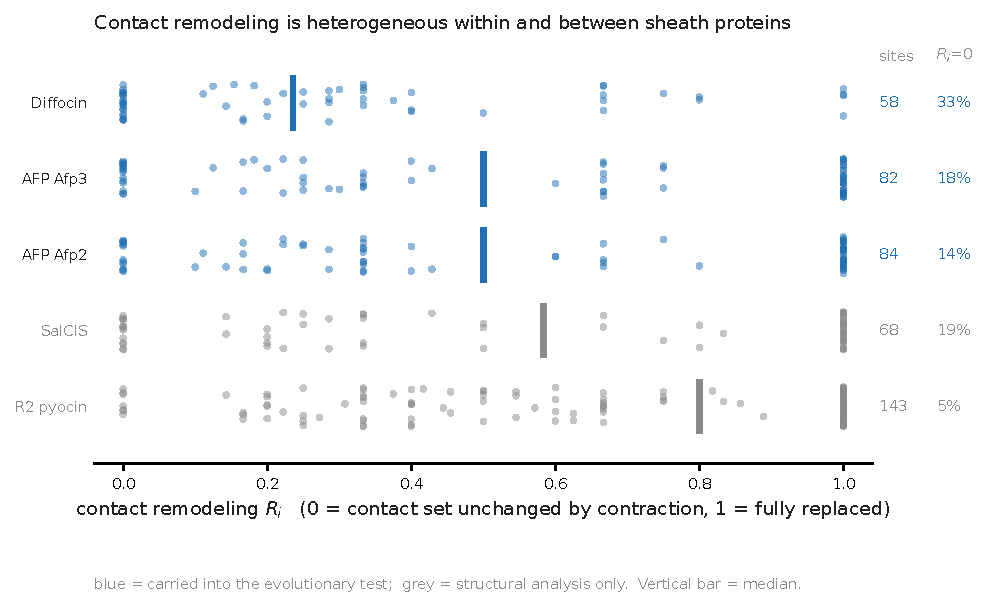
\includegraphics[width=\textwidth,height=0.70\textheight,keepaspectratio]{figures/Figure1.pdf}\par\smallskip
\caption{Residue-level contact remodeling across five sheath protein references from four systems. Each point denotes an eligible residue; vertical bars mark medians. Counts and the proportion with \(R_i\) = 0 are shown. Blue denotes the three proteins with retained evolutionary datasets; grey denotes structural-only references. The two AFP proteins belong to one system. The index compares intermolecular contact identities in two observed conformations; it does not locate these contacts on the sheath or quantify force, energy or displacement.}
\label{fig:remodeling}
\end{figure}

\begin{figure}[p]
\centering
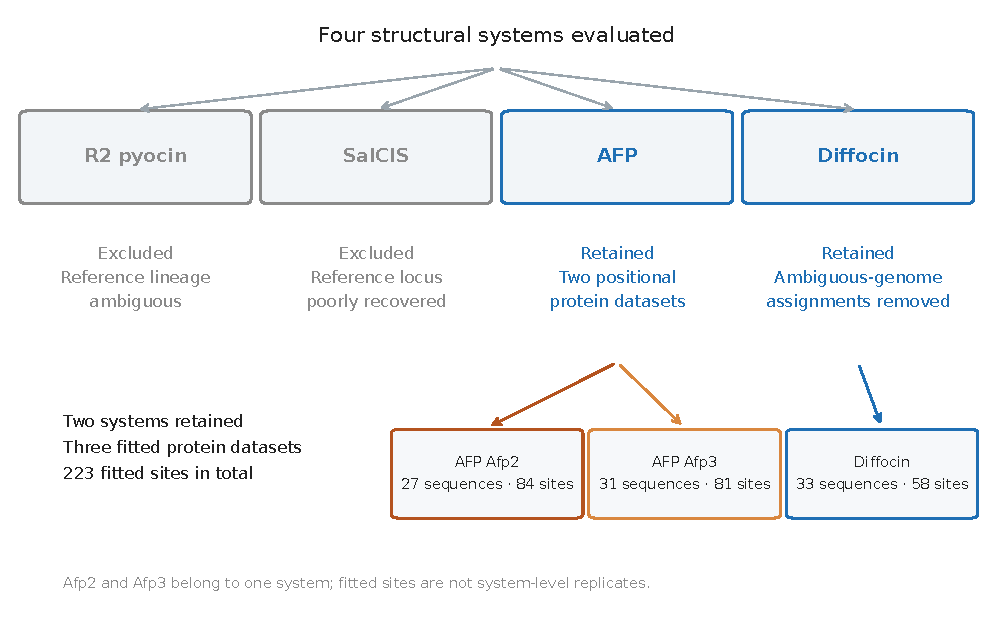
\includegraphics[width=\textwidth,height=0.70\textheight,keepaspectratio]{figures/Figure2.pdf}\par\smallskip
\caption{Evolutionary dataset selection. Four systems were evaluated; positional correspondence supported AFP and diffocin, producing three protein datasets. R2 pyocin was excluded because divergent coexisting copies could not be assigned to one reference lineage, and SalCIS because reference-locus recovery was inadequate. Counts refer to primary sequences and fitted sites, not independent system-level replicates.}
\label{fig:datasets}
\end{figure}

\begin{figure}[p]
\centering
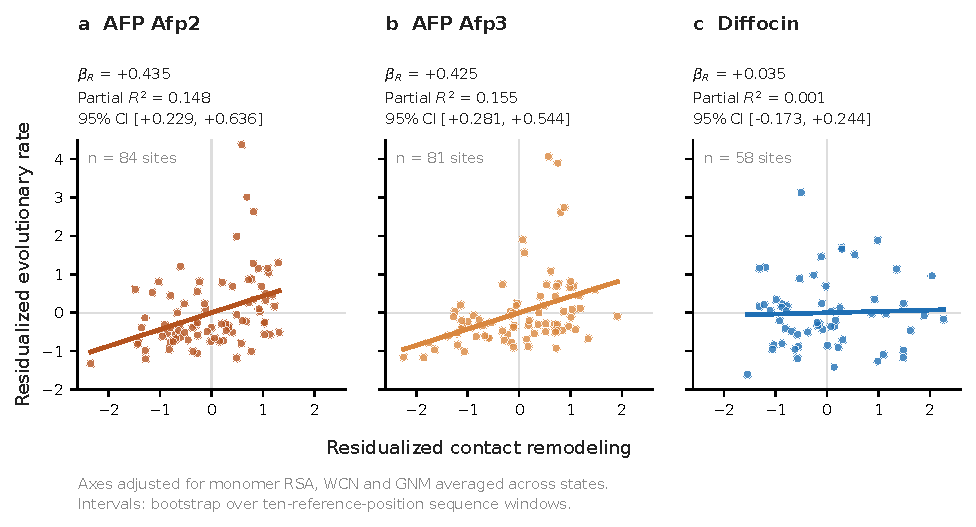
\includegraphics[width=\textwidth,height=0.70\textheight,keepaspectratio]{figures/Figure3.pdf}\par\smallskip
\caption{Added-variable plots for (a) AFP Afp2, (b) AFP Afp3 and (c) diffocin. Both axes are residuals after adjustment of the within-protein standardized variable for RSA, WCN and GNM averaged across states. Points are individual fitted residues. Each line uses the saved full-model standardized remodeling coefficient and was checked against the slope of the saved residuals. Labels report \(\beta_R\), partial \(R^2\) and the 95\% sequence-block-bootstrap interval. These are adjusted relationships, not raw correlations or causal estimates. Intervals use ten-reference-position sequence windows and do not explicitly model three-dimensional structural dependence.}
\label{fig:association}
\end{figure}

\clearpage

\begin{thebibliography}{99}

\bibitem{ref1}
Ge P, Scholl D, Leiman PG, Yu X, Miller JF, Zhou ZH. Atomic structures of a bactericidal contractile nanotube in its pre- and postcontraction states. \emph{Nat Struct Mol Biol}. 2015;22(5):377--382. doi:\href{https://doi.org/10.1038/nsmb.2995}{10.1038/nsmb.2995}.

\bibitem{ref2}
Desfosses A, Venugopal H, Joshi T, et al. Atomic structures of an entire contractile injection system in both the extended and contracted states. \emph{Nat Microbiol}. 2019;4(11):1885--1894. doi:\href{https://doi.org/10.1038/s41564-019-0530-6}{10.1038/s41564-019-0530-6}.

\bibitem{ref3}
Cai X, He Y, Yu I, et al. Atomic structures of a bacteriocin targeting Gram-positive bacteria. \emph{Nat Commun}. 2024;15(1):7057. doi:\href{https://doi.org/10.1038/s41467-024-51038-w}{10.1038/s41467-024-51038-w}.

\bibitem{ref4}
Ejaz RN, Funke K, Kielkopf CS, et al. Structure of a contractile injection system in \emph{Salmonella enterica} subsp. \emph{salamae}. \emph{Nat Commun}. 2026;17:5272. doi:\href{https://doi.org/10.1038/s41467-026-71989-6}{10.1038/s41467-026-71989-6}.

\bibitem{ref5}
Franzosa EA, Xia Y. Structural determinants of protein evolution are context-sensitive at the residue level. \emph{Mol Biol Evol}. 2009;26(10):2387--2395. doi:\href{https://doi.org/10.1093/molbev/msp146}{10.1093/molbev/msp146}.

\bibitem{ref6}
Yeh SW, Huang TT, Liu JW, et al. Local packing density is the main structural determinant of the rate of protein sequence evolution at site level. \emph{Biomed Res Int}. 2014;2014:572409. doi:\href{https://doi.org/10.1155/2014/572409}{10.1155/2014/572409}.

\bibitem{ref7}
Huang TT, del Valle Marcos ML, Hwang JK, Echave J. A mechanistic stress model of protein evolution accounts for site-specific evolutionary rates and their relationship with packing density and flexibility. \emph{BMC Evol Biol}. 2014;14:78. doi:\href{https://doi.org/10.1186/1471-2148-14-78}{10.1186/1471-2148-14-78}.

\bibitem{ref8}
Pupko T, Bell RE, Mayrose I, Glaser F, Ben-Tal N. Rate4Site: an algorithmic tool for the identification of functional regions in proteins by surface mapping of evolutionary determinants within their homologues. \emph{Bioinformatics}. 2002;18(suppl 1):S71--S77. doi:\href{https://doi.org/10.1093/bioinformatics/18.suppl_1.S71}{10.1093/bioinformatics/18.suppl\_1.S71}.

\bibitem{ref9}
Mayrose I, Graur D, Ben-Tal N, Pupko T. Comparison of site-specific rate-inference methods for protein sequences: empirical Bayesian methods are superior. \emph{Mol Biol Evol}. 2004;21(9):1781--1791. doi:\href{https://doi.org/10.1093/molbev/msh194}{10.1093/molbev/msh194}.

\bibitem{ref10}
Paysan-Lafosse T, Andreeva A, Blum M, et al. The Pfam protein families database: embracing AI/ML. \emph{Nucleic Acids Res}. 2025;53(D1):D523--D534. doi:\href{https://doi.org/10.1093/nar/gkae997}{10.1093/nar/gkae997}.

\bibitem{ref11}
UniProt Consortium. UniProt: the Universal Protein Knowledgebase in 2025. \emph{Nucleic Acids Res}. 2025;53(D1):D609--D617. doi:\href{https://doi.org/10.1093/nar/gkae1010}{10.1093/nar/gkae1010}.

\bibitem{ref12}
Camacho C, Coulouris G, Avagyan V, et al. BLAST+: architecture and applications. \emph{BMC Bioinformatics}. 2009;10:421. doi:\href{https://doi.org/10.1186/1471-2105-10-421}{10.1186/1471-2105-10-421}.

\bibitem{ref13}
Deorowicz S, Debudaj-Grabysz A, Gudy\'{s} A. FAMSA: fast and accurate multiple sequence alignment of huge protein families. \emph{Sci Rep}. 2016;6:33964. doi:\href{https://doi.org/10.1038/srep33964}{10.1038/srep33964}.

\bibitem{ref14}
Wong TKF, Ly-Trong N, Ren H, et al. IQ-TREE 3: phylogenomic inference software using complex evolutionary models. \emph{Mol Biol Evol}. 2026;43(5):msag117. doi:\href{https://doi.org/10.1093/molbev/msag117}{10.1093/molbev/msag117}.

\bibitem{ref15}
Kalyaanamoorthy S, Minh BQ, Wong TKF, von Haeseler A, Jermiin LS. ModelFinder: fast model selection for accurate phylogenetic estimates. \emph{Nat Methods}. 2017;14(6):587--589. doi:\href{https://doi.org/10.1038/nmeth.4285}{10.1038/nmeth.4285}.

\bibitem{ref16}
Hoang DT, Chernomor O, von Haeseler A, Minh BQ, Vinh LS. UFBoot2: improving the ultrafast bootstrap approximation. \emph{Mol Biol Evol}. 2018;35(2):518--522. doi:\href{https://doi.org/10.1093/molbev/msx281}{10.1093/molbev/msx281}.

\bibitem{ref17}
Guindon S, Dufayard JF, Lefort V, Anisimova M, Hordijk W, Gascuel O. New algorithms and methods to estimate maximum-likelihood phylogenies: assessing the performance of PhyML 3.0. \emph{Syst Biol}. 2010;59(3):307--321. doi:\href{https://doi.org/10.1093/sysbio/syq010}{10.1093/sysbio/syq010}.

\bibitem{ref18}
Whelan S, Goldman N. A general empirical model of protein evolution derived from multiple protein families using a maximum-likelihood approach. \emph{Mol Biol Evol}. 2001;18(5):691--699. doi:\href{https://doi.org/10.1093/oxfordjournals.molbev.a003851}{10.1093/oxfordjournals.molbev.a003851}.

\bibitem{ref19}
Shrake A, Rupley JA. Environment and exposure to solvent of protein atoms. Lysozyme and insulin. \emph{J Mol Biol}. 1973;79(2):351--371. doi:\href{https://doi.org/10.1016/0022-2836(73)90011-9}{10.1016/0022-2836(73)90011-9}.

\bibitem{ref20}
Tien MZ, Meyer AG, Sydykova DK, Spielman SJ, Wilke CO. Maximum allowed solvent accessibilities of residues in proteins. \emph{PLoS One}. 2013;8(11):e80635. doi:\href{https://doi.org/10.1371/journal.pone.0080635}{10.1371/journal.pone.0080635}.

\bibitem{ref21}
Bahar I, Atilgan AR, Erman B. Direct evaluation of thermal fluctuations in proteins using a single-parameter harmonic potential. \emph{Fold Des}. 1997;2(3):173--181. doi:\href{https://doi.org/10.1016/S1359-0278(97)00024-2}{10.1016/S1359-0278(97)00024-2}.

\bibitem{ref22}
Efron B. Bootstrap methods: another look at the jackknife. \emph{Ann Stat}. 1979;7(1):1--26. doi:\href{https://doi.org/10.1214/aos/1176344552}{10.1214/aos/1176344552}.

\bibitem{ref23}
K\"{u}nsch HR. The jackknife and the bootstrap for general stationary observations. \emph{Ann Stat}. 1989;17(3):1217--1241. doi:\href{https://doi.org/10.1214/aos/1176347265}{10.1214/aos/1176347265}.

\end{thebibliography}

\clearpage

% Included after the main bibliography; supplementary citations use its reference keys.
\section*{Supplementary Methods and Results}
\setcounter{section}{0}
\setcounter{subsection}{0}
\setcounter{table}{0}
\setcounter{figure}{0}
\renewcommand{\thesection}{S\arabic{section}}
\renewcommand{\thetable}{S\arabic{table}}
\renewcommand{\thefigure}{S\arabic{figure}}
\renewcommand{\theHsection}{supp.\arabic{section}}
\renewcommand{\theHtable}{supp.\arabic{table}}
\renewcommand{\theHfigure}{supp.\arabic{figure}}


Anthony Yua Ior, Istanbul Technical University, Maslak 34867, Istanbul, Turkiye. Correspondence: \href{mailto:ior23@itu.edu.tr}{ior23@itu.edu.tr}.

This supplement reports retained outputs and reproducibility details for the three-protein analysis. It does not introduce new rate estimates, model fits or structural calculations. The complete-precision tables, residue mappings, commands and selected archived outputs are supplied in \path{supplementary_data/}. Public repository deposition remains pending.

\section{Supplementary Methods}

\subsection{Structural coordinates, mappings and eligibility}

All five references have both experimental states and complete adjacent-ring shells in the stored structural QC. Canonical indices are zero-based, consecutively assigned to aligned cross-state residue pairs (gapped segments receive no index); \path{seqres_pos} is one-based extended entity sequence position. The residue-mapping CSV preserves author residue numbers in both states, canonical indices, contact counts, eligibility and descriptor values for every recorded position. Gaps and unresolved residues are not assigned coordinates. The two author chain sets are case-sensitive; operator-derived AFP copies are distinct from the deposited chain names. A selected contact-reference subunit key was not archived.

The implementation prefers non-terminal family subunits and then the candidate with the largest number of subunit centroids at strictly less than 90 \AA{}. Python \path{max} retains the first candidate in input order when scores tie. The original mmCIF bytes, selected keys, candidate scores and tie counts are absent, so exact historical subunits cannot be verified from the archived outputs. The accompanying \path{REPRODUCIBILITY_AUDIT.md} documents the ordered-input procedure and separates downstream input replay from structural reconstruction. Residue correspondence uses global BLOSUM62 alignment with opening \ensuremath{-}11 and extension \ensuremath{-}1. Modeled amino acids require C\ensuremath{\alpha}; family matching requires at least 90\% identity, calculated as the number of identical aligned pairs divided by the shorter modeled sequence length. Cross-state mismatches remain aligned when the family meets this criterion. The continuous producer does not implement an engineering mask or the earlier pilot's 8 \AA{} exclusion. Thus neither an engineering exclusion nor a specific unlogged central chain is claimed. Direct PDB chain examples in the main table identify family membership rather than the computational reference copy.

R2, SalCIS and diffocin use deposited copies; AFP applies deposited biological-assembly operators in both states. No retained reference needs guessed screw-based ring completion. The producer's generated-contact flag detects ring-completion keys, rather than all operator-derived coordinates. Its zero value must not be used to deny AFP operator expansion. Contact identity includes partner family, relative ring, relative azimuth modulo inferred ring multiplicity and canonical partner residue. Intramonomer pairs are excluded; another copy of the same family is eligible. Only matched partner positions contribute. Primary eligibility requires a contact union of at least three at strictly less than 5 \AA{}.

The archived cutoff and domain sweeps in Figure~\ref{fig:supp1} describe the structural metric only. They were not used to select a rate-association model. Changing the contact cutoff changes both eligible-site composition and mean remodeling; for example, Afp2 means range from 0.49 to 0.62 over the saved 4--6 \AA{} sweep. These records do not support blanket numerical invariance to the cutoff.

\subsection{Retrieval and positional assignment}

UniProtKB release 2026\_03, released 2 September 2026, supplied bacterial Pfam family pools. Reference UniProt identifiers are listed below. Single-query BLAST+ 2.17.0+ searches used E \ensuremath{\leq} \(10^{-5}\), \path{-seg no} and \path{-max_target_seqs 20000}. Candidate gates were 30--90\% identity, at least 80\% query coverage, and a 0.75--1.30 sequence-length ratio. The best bitscore per species was retained. These filters describe a candidate set and do not establish orthology. AFP's 5,470 joint prescreen records and 279 reference-subfamily screened members are a separate route; missing single-query funnel stages are not replaced by inferred counts.

Annotated genomic neighbourhoods extend \ensuremath{\pm}25 kb around a candidate. Flanking CDS homology was searched against the reference neighbourhood using BLAST with E \ensuremath{\leq} \(10^{-5}\), \path{-max_target_seqs 10} and \path{-seg no}. Sheath genes were excluded from anchoring evidence. Offsets are candidate CDS index minus reference slot. A locus requires at least three non-sheath anchors, at least 60\% support for its modal offset, and collinearity \ensuremath{\rho} \ensuremath{\geq} 0.8 when the collinearity statistic is defined. The retained tables include loci with undefined \ensuremath{\rho}, so this last condition is not a claim that every anchored row carries a finite statistic. Direction was normalized to the sheath orientation, and positional assignment used the modal non-sheath offset. Unanchored or ambiguous positions were left unassigned.

AFP positions 0, 1 and 2 represent Afp2, Afp3 and a third sheath-like gene. Among 42 reference-subfamily loci, 31 were anchored and 35 contained a three-gene run. Across 58 assigned genes in the comparison, 55 agreed with the sequence label. The diagnostic joint FastTree phylogeny has 145 tips, including 85 labeled tips and 60 unassigned tips; the three reference tips are included in those labeled counts. Family-wide labels do not form strictly monophyletic classes. Assignment is supported within the reference subfamily, not by a claim that the joint tree alone establishes universal positional correspondence. The final rate alignments and IQ-TREE topologies are separate from that diagnostic tree.

R2's 5,133 candidate-positive proteomes contain one detected copy in 3,341, two in 1,178, three in 432, four in 99, five in 38, and at least six in 45; the maximum is 20. These are copy counts conditional on the Pfam retrieval and must not be read as an unbiased genome-wide absence screen. Among 25 tested within-genome pairs, ten exceeded the between-genome 90th-percentile distance. The 9,180 between-genome pair distances are not independent observations. Reference-lineage assignment remained ambiguous even in the most diverse single-copy candidate set; no R2 rate regression was performed.

SalCIS's family-wide locus assessment contains 55 loci, nine anchored; 28 contain two sheath-like genes and 27 one. The restricted enterobacterial assessment has 29 loci, nine anchored, with 19 single-, three double- and seven triple-sheath loci. Neither route yields an adequate corresponding reference-position sample. Diffocin has 142 loci with one local sheath gene each, 67 anchored, and 36 exact-offset assignments. Seven of 137 replicons nevertheless contain two candidate loci. Removing both ambiguous \emph{P. hiranonis} assignments gives the primary 33-sequence dataset, distinct from screened 35 and collinear-frame 66 sequence sets.

\subsection{Alignments, trees and rate-estimation settings}

FAMSA through pyfamsa 0.7.0 produced the saved alignments. A separate embedded FAMSA build version was not recorded. No final column trimming is documented. A reference-row gap is skipped when mapping alignment columns to one-based SEQRES positions. Site occupancy is the fraction of rows with a non-gap amino acid. The primary threshold is 80\%; the saved 50\% checks add only one Afp3 site. Invariant columns are retained in primary fits and excluded only in the recorded variable-site checks.

IQ-TREE 3.1.4 used ModelFinder BIC selection, 1,000 ultrafast bootstrap replicates, 1,000 SH-aLRT replicates and four threads. Exact commands and logged random seeds are in \path{archived_commands.txt}. Both AFP topologies selected WAG+I+G4; primary diffocin selected LG+F+I+G4, and both alternative diffocin sets selected Q.PFAM+F+G4. Earlier FastTree 2.2.0 LG+\ensuremath{\Gamma} phylogenies serve orthology/feasibility QC; their summary distances are not substituted for the final IQ-TREE fit.

Rate4Site self-reports version 2.01 although its ConSurf source-directory label is 3.2. The retained build patched three pre-C++11 stream idioms in error and file-open handling, without changes to numerical routines: address comparison in \path{errorMsg.cpp} and \path{!stream.is_open()} checks in \path{someUtil.cpp} and \path{rate4siteOptions.cpp}. Source/build provenance is recorded in \path{FROZEN_ANALYSIS.md}; the build source is retained in the project, not fully reproduced in this compact manuscript bundle. All runs used \path{-Mw -ib -k 16}, a fixed supplied topology (\path{-t}), and reference row \path{-a REF}. Rate4Site reoptimized branch lengths under WAG+\ensuremath{\Gamma}. It implements neither LG nor Q.PFAM, so matrix differences from the selected diffocin topology models are retained and disclosed. The saved IQ-TREE branch lengths remain in the original \path{.treefile} outputs.

Increasing normalized Rate4Site scores mean faster relative evolution. The output also retains unnormalized posterior rates and uncertainty. Invariant sites receive empirical Bayes estimates rather than a single assigned floor. The JSON field \path{invariant_sites_in_fit} counts sites with zero posterior SD, rather than alignment invariance, and is zero in the primary models. The actual invariant counts are 33, 17 and eight for fitted Afp2, Afp3 and diffocin sites. Table~\ref{tab:supp3} checks distinct non-gap amino acids in the saved alignments at the fitted reference positions. The \path{n_aa} field reports occupancy counts, not amino-acid diversity.

\subsection{Structural covariates and statistical implementation}

Shrake--Rupley uses the Biopython defaults (1.4 \AA{} probe radius and 100 surface points per atom) on an isolated chain; residue ASA is divided by Tien theoretical maximum ASA. WCN sums inverse squared C\ensuremath{\alpha} distances to all other modeled residues in that chain, including sequence neighbours. Self-pairs and squared distances \ensuremath{\leq} \(10^{-6}\) \AA{}\ensuremath{^2} are excluded. GNM uses an adjacency of 0 < d < 7.3 \AA{}, the corresponding Kirchhoff Laplacian and the diagonal of its numerical pseudoinverse. No physical fluctuation scale is inferred. Covariates use the representative chain selected during family matching, rather than the interior subunit selected for assembly contacts. The representative monomer-chain keys were not exported. The producer computes both states and writes the available-state arithmetic mean of descriptor values; it does not average atomic coordinates. Only the averaged \path{rsa}, \path{wcn} and \path{gnm} columns are retained; state-specific intermediate values cannot be checked from the tables. This differs from the written extended-state specification. The manuscript uses the archived inputs and does not choose states or refit.

For each protein, the outcome and four predictors are standardized with sample SD (\path{ddof=1}). OLS includes an intercept and uses the full available eligible sites at the specified occupancy. The partial \(R^2\) compares the full model with RSA/WCN/GNM alone. Saved standard errors, OLS intervals and p-values assume independent sites; scientific interpretation instead emphasizes the sequence-block intervals. The intercept estimate and its SE were not exported. It is centered by construction, but no unarchived intercept inferential statistic is invented in Table~\ref{tab:supp4}.

The bootstrap seed is 20261013. Block identifiers are \path{(seqres_pos - 1) // 10}. Only nonempty windows enter the draw pool; a sampled block contributes its eligible rows, so its row count need not equal ten. Blocks are repeatedly drawn with replacement until the original site count is met or exceeded; the last sampled block is truncated to that count. All variables are re-standardized in each replicate and the coefficient is estimated by least squares. The retained runs used all 10,000 replicates. Percentiles 2.5 and 97.5 yield the intervals. This scheme retains some local sequence dependence, not necessarily dependence between sequence-distant spatial neighbours. Neither full coverage under spatial dependence nor uncertainty from structures, sequence selection, phylogenies or rate posteriors is estimated by this resampling procedure.

The written variable-site sensitivity clause explicitly names Afp2. Parallel Afp3 and diffocin restrictions are present in saved results but not expressly named in that clause. Their timing relative to the clause is not recoverable from the retained record, and they are identified as archived parallel checks. The alternative diffocin sets and 50\% occupancy checks are named in the written plan. No additional regression diagnostics, measurement-error models or between-system effect tests were introduced during writing.

\section{Supplementary Results and Tables}

\subsection{Structural references and residue eligibility}

\begingroup
\footnotesize
\setlength{\tabcolsep}{3pt}
\renewcommand{\arraystretch}{1.2}
\begin{longtable}{>{\raggedright\arraybackslash}p{\dimexpr 0.19\linewidth-2\tabcolsep\relax}>{\raggedright\arraybackslash}p{\dimexpr 0.25\linewidth-2\tabcolsep\relax}>{\raggedright\arraybackslash}p{\dimexpr 0.15\linewidth-2\tabcolsep\relax}>{\raggedright\arraybackslash}p{\dimexpr 0.13\linewidth-2\tabcolsep\relax}>{\raggedright\arraybackslash}p{\dimexpr 0.13\linewidth-2\tabcolsep\relax}>{\raggedright\arraybackslash}p{\dimexpr 0.15\linewidth-2\tabcolsep\relax}}
\caption{Structural references, cross-state modeled sequences and eligibility. E/C denotes extended/contracted; copy counts include both AFP families where deposited operators are applied. Full author chain sets and residue mappings accompany the table.}\label{tab:supp1}\\
\toprule
\textbf{Protein} & \textbf{PDB/entity E/C} & \textbf{Modeled E/C} & \textbf{Identity} & \textbf{Eligible} & \textbf{Copies E/C} \\
\midrule
\endfirsthead
\multicolumn{6}{l}{\tablename~\thetable{} (continued)}\\
\toprule
\textbf{Protein} & \textbf{PDB/entity E/C} & \textbf{Modeled E/C} & \textbf{Identity} & \textbf{Eligible} & \textbf{Copies E/C} \\
\midrule
\endhead
\bottomrule
\endfoot
R2 pyocin & 3J9Q/1 / 3J9R/1 & 385/383 & 1.000 & 143 & 24/36 \\
AFP Afp2 & 6RBN/2 / 6RC8/1 & 350/348 & 1.000 & 84 & 24/48 \\
AFP Afp3 & 6RBN/3 / 6RC8/2 & 358/355 & 0.992 & 82 & 24/48 \\
SalCIS & 9R9H/1 / 9R9I/1 & 514/495 & 0.994 & 68 & 18/18 \\
Diffocin & 8V3X/1 / 8V3Y/1 & 352/353 & 1.000 & 58 & 18/30 \\
\end{longtable}
\endgroup

\textbf{R2 pyocin:} author chains E: A--R, X, a, d, g, j, m; C: 0--5, A--R, a--l. Eligible reference-position range 2--383 (not every intervening position is eligible). Coordinates: deposited copies.

\textbf{AFP Afp2:} author chains E: C; C: A. Eligible reference-position range 5--351 (not every intervening position is eligible). Coordinates: deposited operators.

\textbf{AFP Afp3:} author chains E: D; C: B. Eligible reference-position range 4--447 (not every intervening position is eligible). Coordinates: deposited operators.

\textbf{SalCIS:} author chains E: T--Z, a--k; C: O--Z, a--f. Eligible reference-position range 12--515 (not every intervening position is eligible). Coordinates: deposited copies.

\textbf{Diffocin:} author chains E: E, F, P, Q, S--X, d, e, g, n, q--s, z; C: A--Z, a--d. Eligible reference-position range 3--354 (not every intervening position is eligible). Coordinates: deposited copies.

Full mappings and deposited author chain lists are in the Table~\ref{tab:supp1} CSVs. Selected interior keys are not archived; all five reported shells are complete and no ring completion was required. Paired identities are rounded in the stored outputs.

\subsection{Retrieval counts and orthology decisions}

\begingroup
\footnotesize
\setlength{\tabcolsep}{3pt}
\renewcommand{\arraystretch}{1.2}
\begin{longtable}{>{\raggedright\arraybackslash}p{\dimexpr 0.16\linewidth-2\tabcolsep\relax}>{\raggedright\arraybackslash}p{\dimexpr 0.08\linewidth-2\tabcolsep\relax}>{\raggedright\arraybackslash}p{\dimexpr 0.15\linewidth-2\tabcolsep\relax}>{\raggedright\arraybackslash}p{\dimexpr 0.13\linewidth-2\tabcolsep\relax}>{\raggedright\arraybackslash}p{\dimexpr 0.12\linewidth-2\tabcolsep\relax}>{\raggedright\arraybackslash}p{\dimexpr 0.36\linewidth-2\tabcolsep\relax}}
\caption{Retrieval funnels and orthology decisions. AFP uses a joint prescreen rather than a directly comparable single-query gated funnel. Counts are screening-stage observations.}\label{tab:supp2}\\
\toprule
\textbf{Route} & \textbf{Pool} & \textbf{BLAST/prescreen} & \textbf{Gated} & \textbf{Species} & \textbf{Decision} \\
\midrule
\endfirsthead
\multicolumn{6}{l}{\tablename~\thetable{} (continued)}\\
\toprule
\textbf{Route} & \textbf{Pool} & \textbf{BLAST/prescreen} & \textbf{Gated} & \textbf{Species} & \textbf{Decision} \\
\midrule
\endhead
\bottomrule
\endfoot
R2 pyocin & 8035 & 4593 & 1266 & 967 & excluded: reference lineage ambiguous \\
SalCIS & 7592 & 4490 & 805 & 667 & excluded: reference locus poorly recovered \\
Diffocin & 8005 & 930 & 192 & 165 & retained: primary 33 sequences \\
AFP joint route & 8005 & 5470 & not comparable & not comparable & retained: Afp2 27 / Afp3 31 \\
\end{longtable}
\endgroup

Reference sequence identifiers: r2pyocin: Q9S574 (386 aa), Pfam PF04984, PF17482, PF22671; afp\_Afp2: Q6HAD7 (354 aa), Pfam PF04984, PF17482; afp\_Afp3: Q6HAD6 (451 aa), Pfam PF04984, PF17482; salcis: A0A701XPN5 (519 aa), Pfam PF17482; diffocin: A0A9Q7ZU73 (354 aa), Pfam PF04984, PF17482.

Counts describe recorded screening stages rather than final interchangeable ortholog sets. The AFP prescreen differs from the three single-query routes. Family-wide AFP diagnosis and reference-subfamily selection are separate. Detailed locus records are retained in the project; Figures S2--S4 summarize selected archived evidence.

\subsection{Final alignment occupancy and variability}

\begingroup
\footnotesize
\setlength{\tabcolsep}{3pt}
\renewcommand{\arraystretch}{1.2}
\begin{longtable}{>{\raggedright\arraybackslash}p{\dimexpr 0.26\linewidth-2\tabcolsep\relax}>{\raggedright\arraybackslash}p{\dimexpr 0.13\linewidth-2\tabcolsep\relax}>{\raggedright\arraybackslash}p{\dimexpr 0.14\linewidth-2\tabcolsep\relax}>{\raggedright\arraybackslash}p{\dimexpr 0.16\linewidth-2\tabcolsep\relax}>{\raggedright\arraybackslash}p{\dimexpr 0.12\linewidth-2\tabcolsep\relax}>{\raggedright\arraybackslash}p{\dimexpr 0.19\linewidth-2\tabcolsep\relax}}
\caption{Alignment metadata, fitted-site occupancy and variability. Values come from saved alignments and site tables; the alternate diffocin sets are sensitivity datasets.}\label{tab:supp3}\\
\toprule
\textbf{Dataset} & \textbf{Sequences} & \textbf{Columns} & \textbf{Fitted sites} & \textbf{Variable} & \textbf{Minimum occupancy} \\
\midrule
\endfirsthead
\multicolumn{6}{l}{\tablename~\thetable{} (continued)}\\
\toprule
\textbf{Dataset} & \textbf{Sequences} & \textbf{Columns} & \textbf{Fitted sites} & \textbf{Variable} & \textbf{Minimum occupancy} \\
\midrule
\endhead
\bottomrule
\endfoot
AFP Afp2 & 27 & 415 & 84 & 51 & 1.000 \\
AFP Afp3 & 31 & 708 & 81 & 64 & 0.903 \\
Diffocin & 33 & 515 & 58 & 50 & 0.970 \\
diffocin asscreened & 35 & 535 & 58 & 50 & 0.971 \\
diffocin collinear & 66 & 565 & 58 & 53 & 0.985 \\
\end{longtable}
\endgroup

Fitted-site counts use the retained primary or alternative site tables. Afp3 has 82 structural sites, of which one has 0.742 occupancy and is excluded at 80\%. Its 81-site primary model has 64 variable sites; the 82-site occupancy sensitivity has 65. All Afp2 structural sites have full occupancy. Primary diffocin structural sites have minimum occupancy 0.970. The supplied CSV records exact alignment paths and reference lengths.

Taxonomic breadth (effective genera) is 5.49 for Afp2, 5.43 for Afp3, 16.71 for primary diffocin, 17.71 for screened diffocin and 31.27 for collinear diffocin. AFP spans eight genera; the largest genus contributes 33.3\% and 32.3\%, respectively. Primary diffocin contains 29 species in 20 genera and its largest genus contributes 12.5\%. These are sampling summaries, not numbers of independent evolutionary replicates.

Earlier AFP feasibility trees have total lengths 6.62 and 17.02 substitutions per site, mean patristic distances 0.914 and 1.937, and maximum distances 1.683 and 5.550. The historical screened 35-sequence diffocin tree has total length 16.18, mean distance 1.592 and maximum 2.444. These QC summaries are not final IQ-TREE summaries and the 35-sequence values must not be relabeled as properties of the 33-sequence primary tree. The retained R2 best single-copy set had 136 sequences, 143 sites, eight invariant sites, effective genera 22.25 and a maximum QC patristic distance of 4.207, but was excluded on orthology rather than diversity grounds. No corresponding SalCIS rate dataset was constructed.

\subsection{Full exported primary regression coefficients}

\begingroup
\footnotesize
\setlength{\tabcolsep}{3pt}
\renewcommand{\arraystretch}{1.2}
\begin{longtable}{>{\raggedright\arraybackslash}p{\dimexpr 0.16\linewidth-2\tabcolsep\relax}>{\raggedright\arraybackslash}p{\dimexpr 0.1\linewidth-2\tabcolsep\relax}>{\raggedright\arraybackslash}p{\dimexpr 0.1\linewidth-2\tabcolsep\relax}>{\raggedright\arraybackslash}p{\dimexpr 0.1\linewidth-2\tabcolsep\relax}>{\raggedright\arraybackslash}p{\dimexpr 0.23\linewidth-2\tabcolsep\relax}>{\raggedright\arraybackslash}p{\dimexpr 0.1\linewidth-2\tabcolsep\relax}>{\raggedright\arraybackslash}p{\dimexpr 0.11\linewidth-2\tabcolsep\relax}}
\caption{All exported non-intercept primary coefficients, independent-site OLS standard errors, intervals and p-values, and variance inflation factors. Intercept inferential statistics were not exported.}\label{tab:supp4}\\
\toprule
\textbf{Protein} & \textbf{Predictor} & \textbf{\ensuremath{\beta}} & \textbf{SE} & \textbf{OLS 95\% CI} & \textbf{OLS p} & \textbf{VIF} \\
\midrule
\endfirsthead
\multicolumn{7}{l}{\tablename~\thetable{} (continued)}\\
\toprule
\textbf{Protein} & \textbf{Predictor} & \textbf{\ensuremath{\beta}} & \textbf{SE} & \textbf{OLS 95\% CI} & \textbf{OLS p} & \textbf{VIF} \\
\midrule
\endhead
\bottomrule
\endfoot
AFP Afp2 & R & +0.4351 & 0.1176 & [+0.2010, +0.6692] & 0.0003978 & 1.412 \\
AFP Afp2 & rsa & +0.2114 & 0.1420 & [-0.0712, +0.4939] & 0.1404 & 2.056 \\
AFP Afp2 & wcn & +0.2654 & 0.2212 & [-0.1749, +0.7057] & 0.2338 & 4.994 \\
AFP Afp2 & gnm & +0.1367 & 0.2089 & [-0.2790, +0.5525] & 0.5147 & 4.452 \\
AFP Afp3 & R & +0.4247 & 0.1136 & [+0.1983, +0.6510] & 0.0003582 & 1.241 \\
AFP Afp3 & rsa & +0.1947 & 0.1487 & [-0.1014, +0.4908] & 0.1942 & 2.123 \\
AFP Afp3 & wcn & +0.3290 & 0.2209 & [-0.1109, +0.7688] & 0.1405 & 4.687 \\
AFP Afp3 & gnm & +0.2791 & 0.2028 & [-0.1248, +0.6831] & 0.1728 & 3.952 \\
Diffocin & R & +0.0347 & 0.1354 & [-0.2369, +0.3063] & 0.7988 & 1.105 \\
Diffocin & rsa & +0.1341 & 0.2294 & [-0.3260, +0.5942] & 0.5612 & 3.172 \\
Diffocin & wcn & -0.5623 & 0.3731 & [-1.3107, +0.1862] & 0.1378 & 8.392 \\
Diffocin & gnm & -0.5451 & 0.2896 & [-1.1261, +0.0358] & 0.06531 & 5.056 \\
\end{longtable}
\endgroup

All four non-intercept coefficients are standardized within protein. Independent-site OLS statistics are descriptive; primary remodeling inference uses the block-bootstrap intervals in main Table~\ref{tab:primary}. Intercept inferential statistics were not archived. VIFs indicate appreciable collinearity among conventional descriptors despite relatively low VIF for remodeling. Full-precision values are preserved in the supplied CSV and original JSON.

\subsection{Complete archived sensitivity results}

\clearpage
\begin{landscape}
\begingroup
\footnotesize
\setlength{\tabcolsep}{3pt}
\renewcommand{\arraystretch}{1.2}
\begin{longtable}{>{\raggedright\arraybackslash}p{\dimexpr 0.22\linewidth-2\tabcolsep\relax}>{\raggedright\arraybackslash}p{\dimexpr 0.09\linewidth-2\tabcolsep\relax}>{\raggedright\arraybackslash}p{\dimexpr 0.07\linewidth-2\tabcolsep\relax}>{\raggedright\arraybackslash}p{\dimexpr 0.08\linewidth-2\tabcolsep\relax}>{\raggedright\arraybackslash}p{\dimexpr 0.07\linewidth-2\tabcolsep\relax}>{\raggedright\arraybackslash}p{\dimexpr 0.09\linewidth-2\tabcolsep\relax}>{\raggedright\arraybackslash}p{\dimexpr 0.18\linewidth-2\tabcolsep\relax}>{\raggedright\arraybackslash}p{\dimexpr 0.1\linewidth-2\tabcolsep\relax}>{\raggedright\arraybackslash}p{\dimexpr 0.1\linewidth-2\tabcolsep\relax}}
\caption{Complete archived sensitivity results. An asterisk marks Afp3 and diffocin variable-site checks beyond the literal Afp2-only written clause. Other specifications are named in the written sensitivity plan. Bootstrap intervals follow the primary sequence-window scheme.}\label{tab:supp5}\\
\toprule
\textbf{Specification} & \textbf{Sequences} & \textbf{Sites} & \textbf{\(\beta_R\)} & \textbf{SE} & \textbf{OLS p} & \textbf{Sequence-block 95\% CI} & \textbf{Partial \(R^2\)} & \textbf{Full \(R^2\)} \\
\midrule
\endfirsthead
\multicolumn{9}{l}{\tablename~\thetable{} (continued)}\\
\toprule
\textbf{Specification} & \textbf{Sequences} & \textbf{Sites} & \textbf{\(\beta_R\)} & \textbf{SE} & \textbf{OLS p} & \textbf{Sequence-block 95\% CI} & \textbf{Partial \(R^2\)} & \textbf{Full \(R^2\)} \\
\midrule
\endhead
\bottomrule
\endfoot
Diffocin screened & 35 & 58 & +0.0707 & 0.1358 & 0.6048 & [-0.1516, +0.3016] & 0.0051 & 0.1157 \\
Diffocin collinear & 66 & 58 & +0.1208 & 0.1372 & 0.3827 & [-0.1183, +0.3610] & 0.0144 & 0.0977 \\
Afp2 variable & 27 & 51 & +0.2748 & 0.1712 & 0.1153 & [-0.0228, +0.5446] & 0.0531 & 0.1981 \\
Afp3 variable* & 31 & 64 & +0.3550 & 0.1526 & 0.02344 & [+0.1893, +0.4902] & 0.0840 & 0.1691 \\
Diffocin variable* & 33 & 50 & -0.0589 & 0.1475 & 0.6916 & [-0.3390, +0.2338] & 0.0035 & 0.1196 \\
Diffocin occupancy 50\% & 33 & 58 & +0.0347 & 0.1354 & 0.7988 & [-0.1734, +0.2441] & 0.0012 & 0.1207 \\
Afp2 occupancy 50\% & 27 & 84 & +0.4351 & 0.1176 & 0.0003978 & [+0.2286, +0.6360] & 0.1476 & 0.2258 \\
Afp3 occupancy 50\% & 31 & 82 & +0.4190 & 0.1122 & 0.0003567 & [+0.2773, +0.5411] & 0.1535 & 0.2123 \\
\end{longtable}
\endgroup
\end{landscape}

An asterisk identifies parallel variable-site checks beyond the literal Afp2-only clause. The other rows correspond to named sensitivity specifications. These results are unchanged from the saved JSON; rounded CSVs are not used as the authoritative coefficient source. Each model retains all three structural covariates and the same sequence-window bootstrap. No association is detected in diffocin in these specifications. Afp2's variable-site interval includes zero, whereas Afp3's parallel restriction retains a positive interval.

\clearpage

\section*{Supplementary Figures}

\begin{figure}[p]
\centering
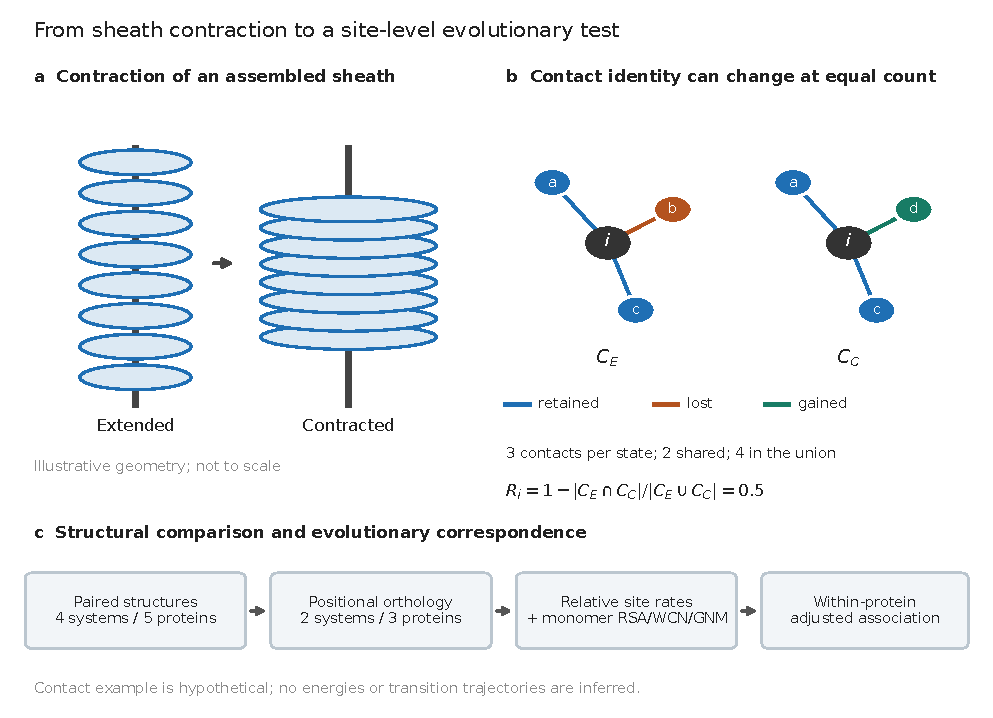
\includegraphics[width=\textwidth,height=0.34\textheight,keepaspectratio]{figures/FigureS1a.pdf}\par\smallskip
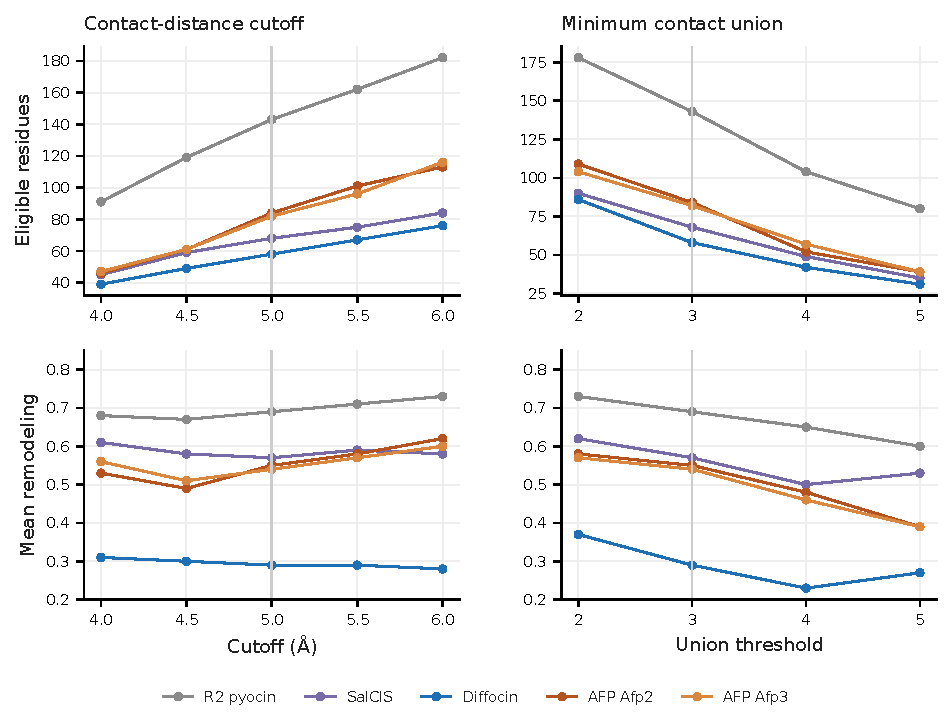
\includegraphics[width=\textwidth,height=0.37\textheight,keepaspectratio]{figures/FigureS1b.pdf}\par\smallskip
\caption{Contact-definition and mapping QC. (a) Explanatory sheath/contact-set schematic; the geometry and contact example are hypothetical and do not represent an atomic rendering. (b) Stored cutoff and union-domain sweeps show eligible-site counts and mean remodeling for the five retained references. These are structural QC summaries from the saved report, not new calculations or evolutionary sensitivity fits.}
\label{fig:supp1}
\end{figure}

\begin{figure}[p]
\centering
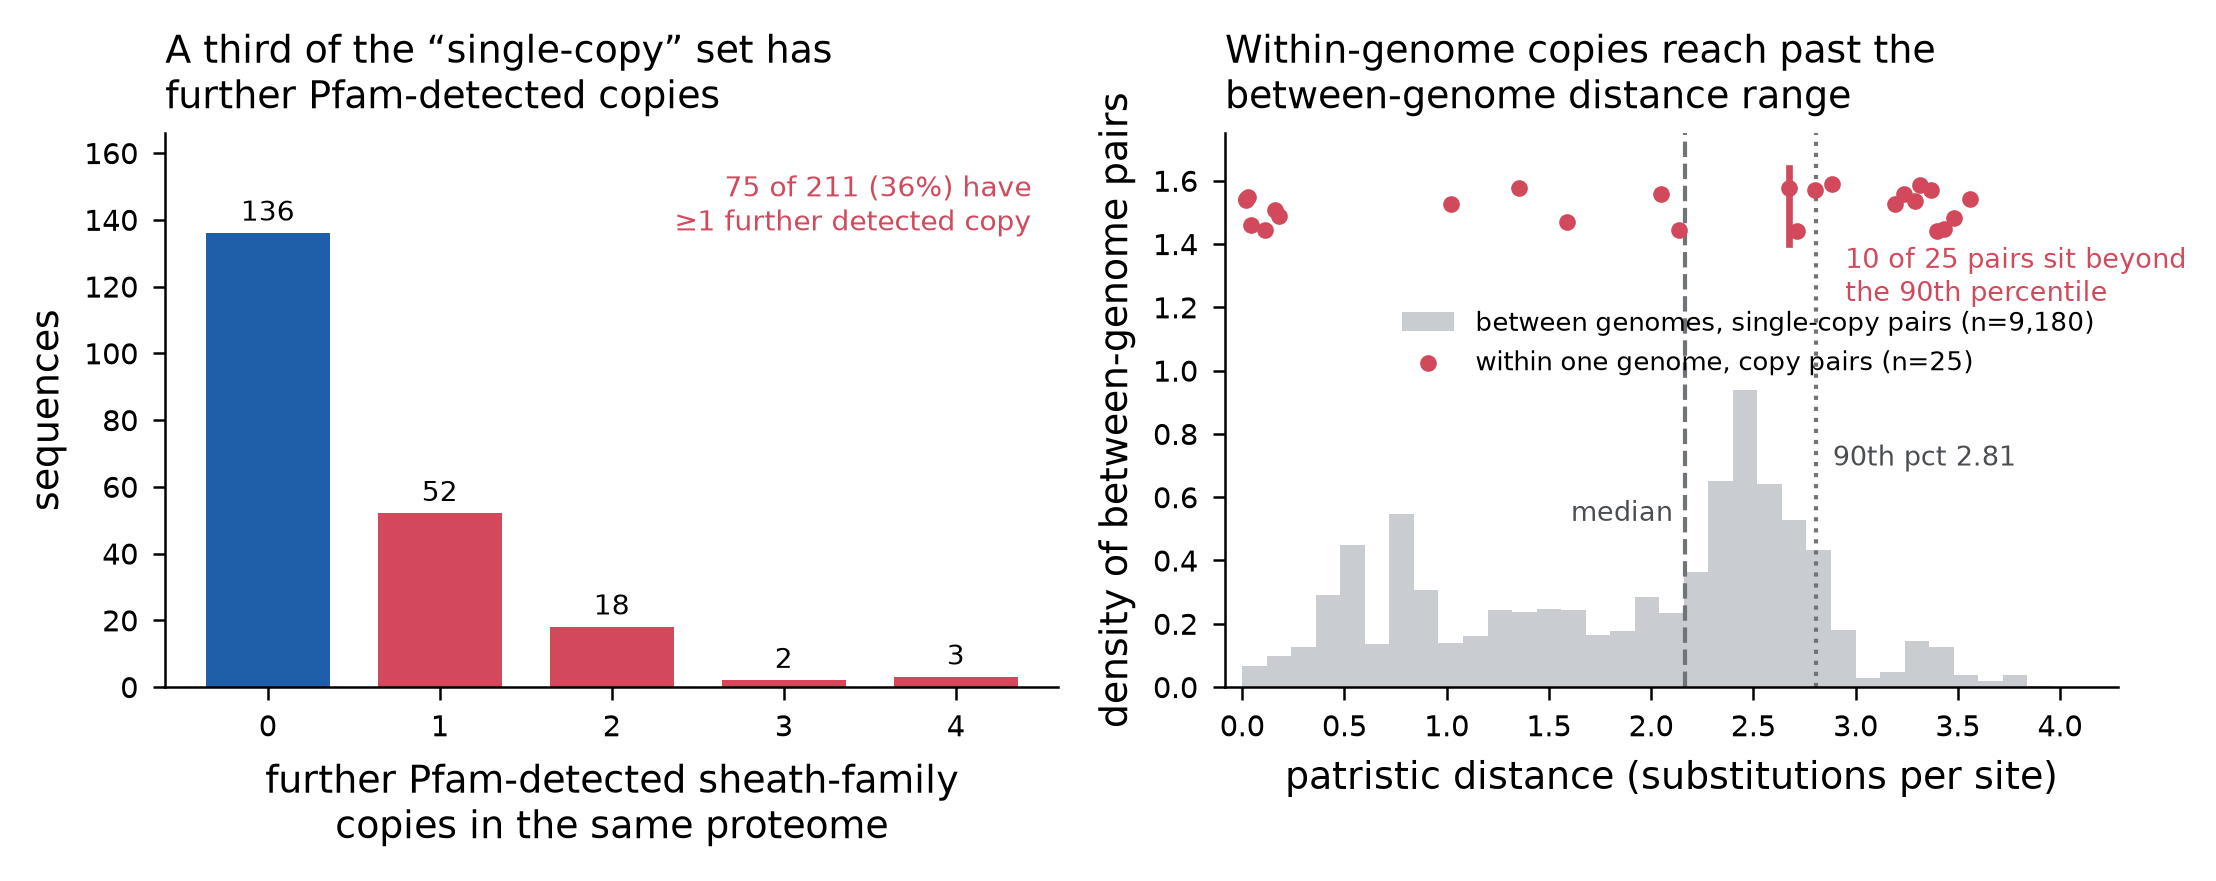
\includegraphics[width=\textwidth,height=0.30\textheight,keepaspectratio]{figures/FigureS2a.png}\par\smallskip
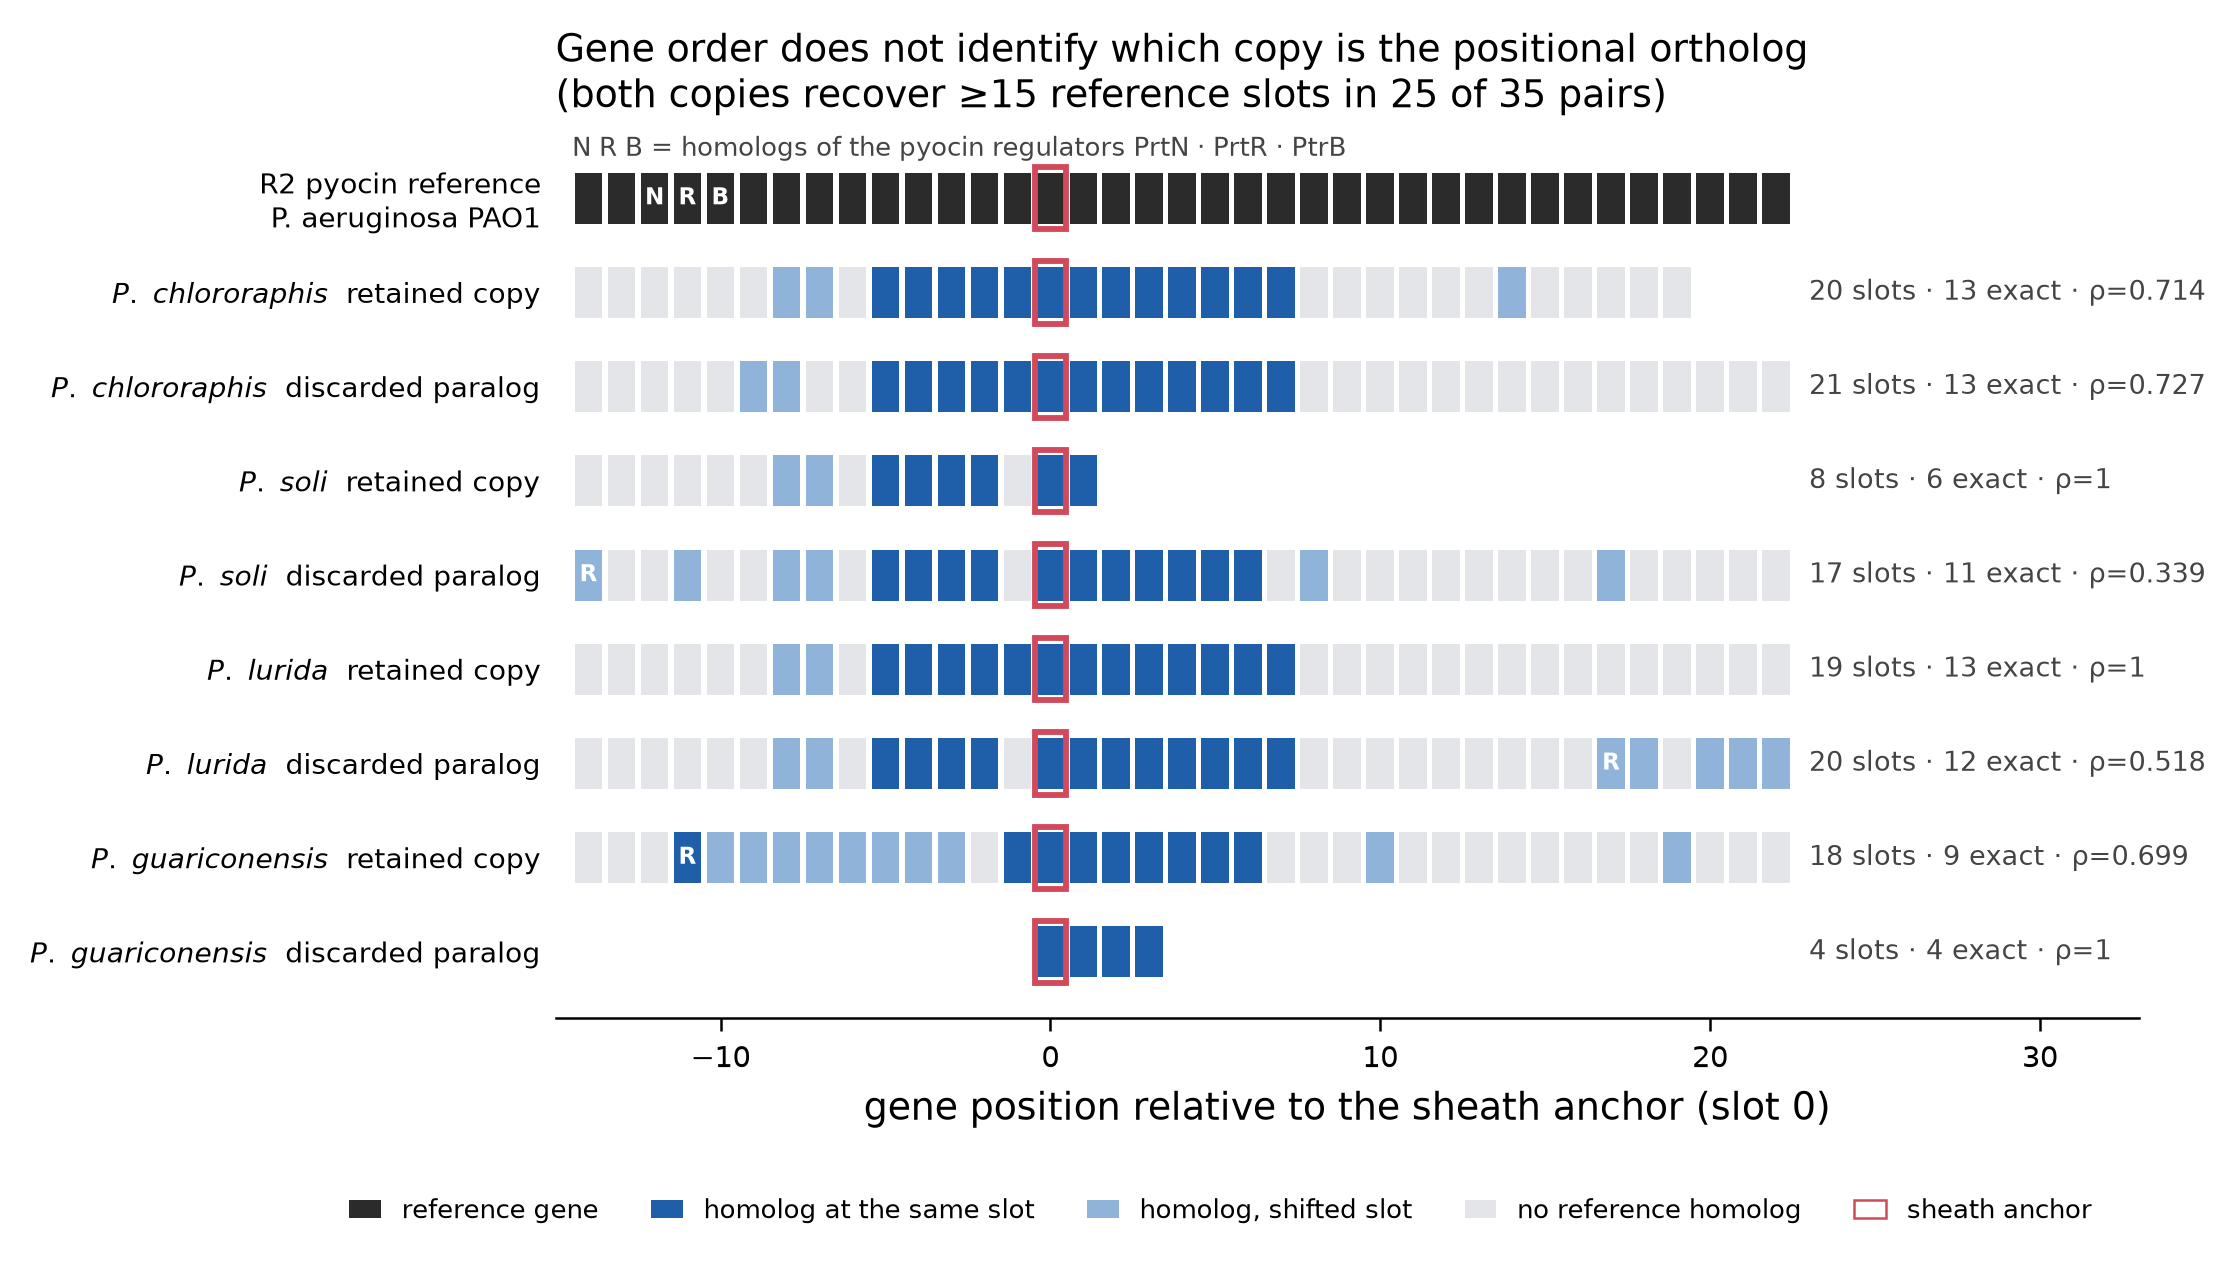
\includegraphics[width=\textwidth,height=0.38\textheight,keepaspectratio]{figures/FigureS2b.png}\par\smallskip
\caption{R2 copy-number and paralogy evidence. (a) The existing copy-number audit and within- versus between-genome distance comparison. Counts are conditional on retrieval; pair distances share sequences and are not independent. (b) Existing retained/discarded candidate locus examples illustrate reference-order ambiguity. These diagnostic candidate sets were not used for a primary rate regression.}
\label{fig:supp2}
\end{figure}

\begin{figure}[p]
\centering
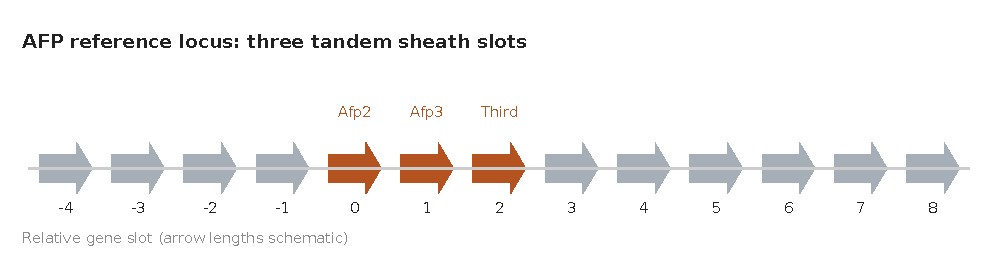
\includegraphics[width=\textwidth,height=0.14\textheight,keepaspectratio]{figures/FigureS3a.pdf}\par\smallskip
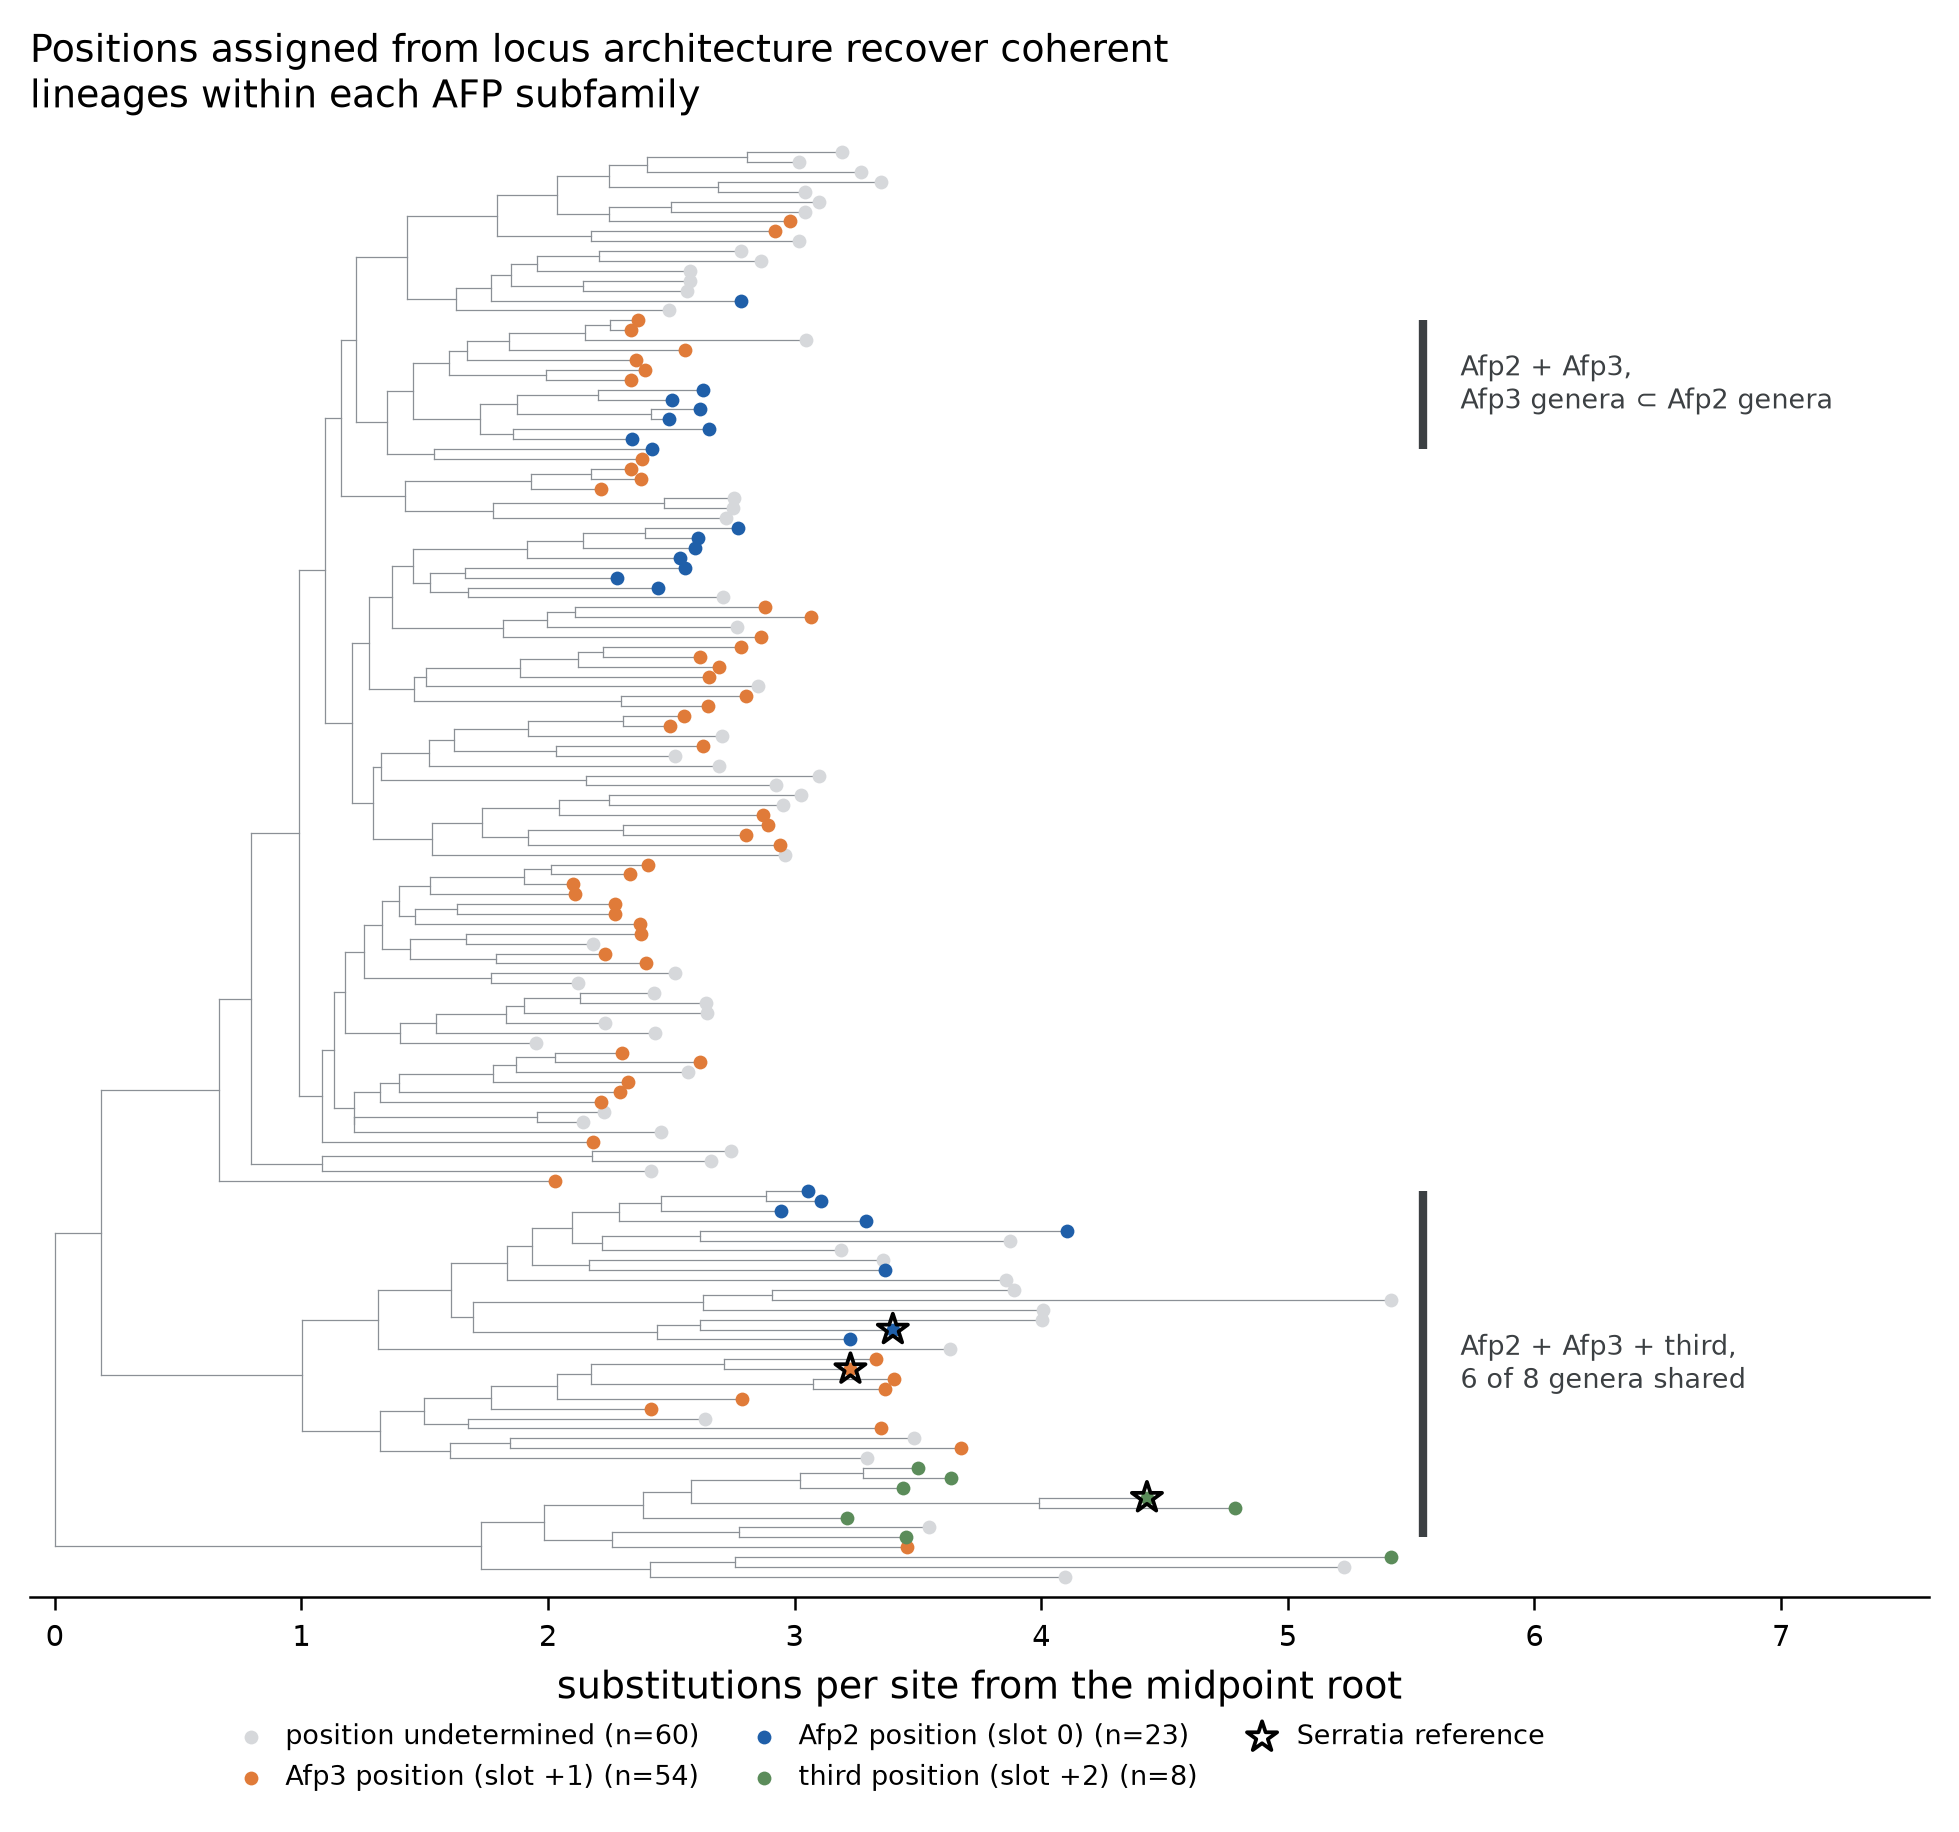
\includegraphics[width=\textwidth,height=0.58\textheight,keepaspectratio]{figures/FigureS3b.png}\par\smallskip
\caption{AFP locus architecture and phylogenetic assignment. (a) Reference-neighbourhood gene order from the saved annotation, oriented relative to the sheath. Arrows show CDS orientation and relative order, not nucleotide lengths; sheath slots 0--2 are highlighted. (b) Existing 145-tip joint FastTree diagnostic phylogeny with positional classes and reference tips. It is distinct from the final protein-specific IQ-TREE rate topologies.}
\label{fig:supp3}
\end{figure}

\begin{figure}[p]
\centering
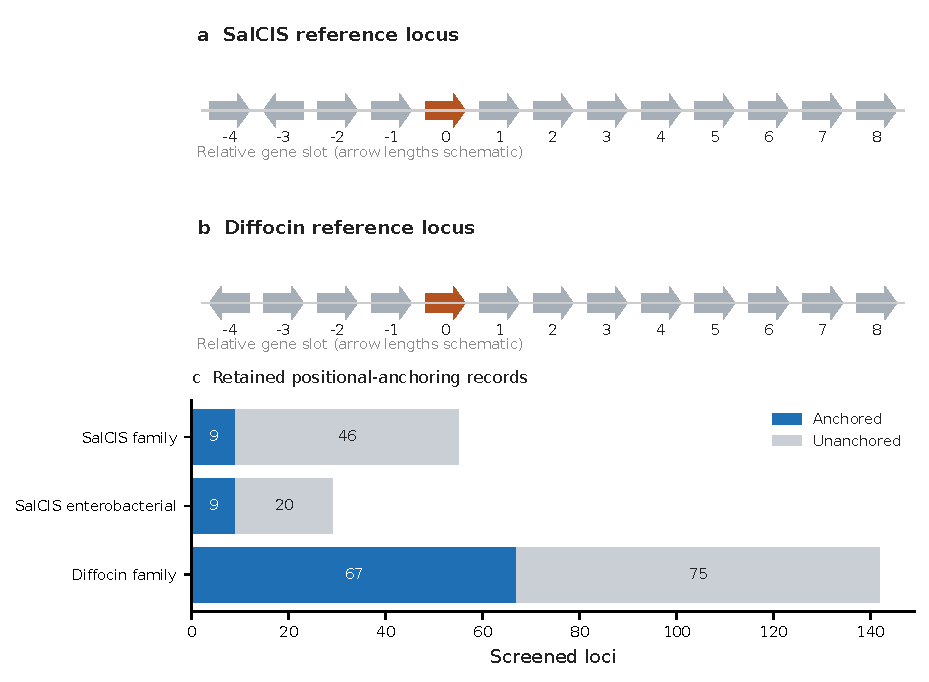
\includegraphics[width=\textwidth,height=0.70\textheight,keepaspectratio]{figures/FigureS4.pdf}\par\smallskip
\caption{SalCIS and diffocin positional evidence. Reference gene order and counts of anchored/unanchored loci are drawn from saved annotation and locus tables. SalCIS shows family-wide and restricted enterobacterial assessments; diffocin shows the family-wide assessment. These screening-stage counts do not equal final rate-dataset sizes. Arrow lengths are schematic. Diffocin's local single-sheath pattern does not rule out multiple loci per replicon.}
\label{fig:supp4}
\end{figure}

\begin{figure}[p]
\centering
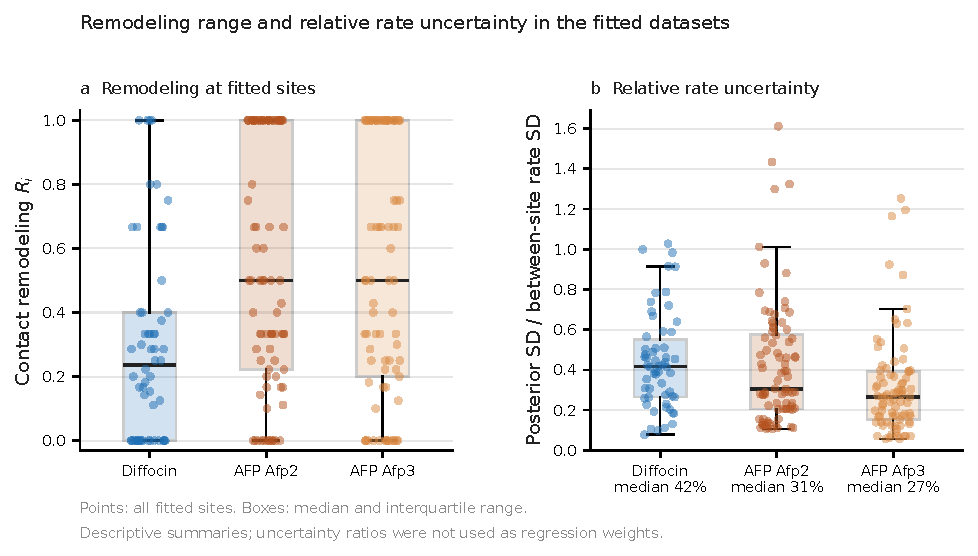
\includegraphics[width=\textwidth,height=0.65\textheight,keepaspectratio]{figures/FigureS5.pdf}\par\smallskip
\caption{Descriptive remodeling range and relative posterior rate uncertainty at the primary fitted sites. Posterior SD is divided by the sample SD of point-estimated rates within each protein. Points and boxes summarize saved site tables. This is an existing descriptive diagnostic, not a new power calculation, uncertainty-propagation model or regression weighting scheme.}
\label{fig:supp5}
\end{figure}


\end{document}
